
\documentclass[a4paper,UKenglish]{lipics-v2018}
%This is a template for producing LIPIcs articles. 
%See lipics-manual.pdf for further information.
%for A4 paper format use option "a4paper", for US-letter use option "letterpaper"
%for british hyphenation rules use option "UKenglish", for american hyphenation rules use option "USenglish"
% for section-numbered lemmas etc., use "numberwithinsect"

\nolinenumbers

\usepackage{microtype}%if unwanted, comment out or use option "draft"

%\graphicspath{{./graphics/}}%helpful if your graphic files are in another directory

\bibliographystyle{plainurl}% the recommnded bibstyle

\title{Typed First-Class Traits}
% \titlerunning{Dummy short title}%optional, please use if title is longer than one line

\author{Xuan Bi}{The University of Hong Kong, Hong Kong, China}{xbi@cs.hku.hk}{}{}%mandatory, please use full name; only 1 author per \author macro; first two parameters are mandatory, other parameters can be empty.

\author{Bruno C. d. S. Oliveira}{The University of Hong Kong, Hong Kong, China}{bruno@cs.hku.hk}{}{}


\authorrunning{X.\,Bi and B.\,C.\,d.\,S.\,Oliveira} %mandatory. First: Use abbreviated first/middle names. Second (only in severe cases): Use first author plus 'et. al.'

\Copyright{Xuan Bi and Bruno C. d. S. Oliveira}%mandatory, please use full first names. LIPIcs license is "CC-BY";  http://creativecommons.org/licenses/by/3.0/


\subjclass{Software and its engineering $\rightarrow$ Object oriented languages}% mandatory: Please choose ACM 2012 classifications from https://www.acm.org/publications/class-2012 or https://dl.acm.org/ccs/ccs_flat.cfm . E.g., cite as "General and reference $\rightarrow$ General literature" or \ccsdesc[100]{General and reference~General literature}.

\keywords{traits, extensible designs}%mandatory

\category{}%optional, e.g. invited paper

\relatedversion{}%optional, e.g. full version hosted on arXiv, HAL, or other respository/website

\supplement{}%optional, e.g. related research data, source code, ... hosted on a repository like zenodo, figshare, GitHub, ...

\funding{Hong Kong Research Grant Council projects number 17210617 and 17258816}%optional, to capture a funding statement, which applies to all authors. Please enter author specific funding statements as fifth argument of the \author macro.

\acknowledgements{We thank the anonymous reviewers for their helpful comments.}%optional

%Editor-only macros:: begin (do not touch as author)%%%%%%%%%%%%%%%%%%%%%%%%%%%%%%%%%%
\EventEditors{Todd Millstein}
\EventNoEds{1}
\EventLongTitle{32nd European Conference on Object-Oriented Programming (ECOOP 2018)}
\EventShortTitle{ECOOP 2018}
\EventAcronym{ECOOP}
\EventYear{2018}
\EventDate{July 16--21, 2018}
\EventLocation{Amsterdam, Netherlands}
\EventLogo{}
\SeriesVolume{109}
\ArticleNo{9} % “New number” (=<article-no>) goes here!%\nolinenumbers %uncomment to disable line numbering
%\hideLIPIcs  %uncomment to remove references to LIPIcs series (logo, DOI, ...), e.g. when preparing a pre-final version to be uploaded to arXiv or another public repository
%%%%%%%%%%%%%%%%%%%%%%%%%%%%%%%%%%%%%%%%%%%%%%%%%%%%%%


% Basics
\usepackage{fixltx2e}
\usepackage{url}
\usepackage{fancyvrb}
\usepackage{mdwlist}  % Miscellaneous list-related commands
\usepackage{xspace}   % Smart spacing
\usepackage{supertabular}
\usepackage{longtable}


% https://www.nesono.com/?q=book/export/html/347
% Package for inserting TODO statements in nice colorful boxes - so that you
% won’t forget to fix/remove them. To add a todo statement, use something like
% \todo{Find better wording here}.
\usepackage{todonotes}

%% Math
\usepackage{amsmath}
\usepackage{amsthm}
\usepackage{amssymb}
\usepackage{bm}       % Bold symbols in maths mode

% http://tex.stackexchange.com/questions/114151/how-do-i-reference-in-appendix-a-theorem-given-in-the-body
\usepackage{thmtools, thm-restate}

%% Theoretical computer science
\usepackage{stmaryrd}
\usepackage{mathtools}  % For "::=" ( \Coloneqq )

%% Font
% \usepackage[euler-digits,euler-hat-accent]{eulervm}


%% Some recommended packages.
\usepackage{booktabs}   %% For formal tables:
                        %% http://ctan.org/pkg/booktabs
\usepackage{subcaption} %% For complex figures with subfigures/subcaptions
                        %% http://ctan.org/pkg/subcaption

% Hyper links
\usepackage{url}
\usepackage{
  nameref,%\nameref
  hyperref,%\autoref
}
\usepackage[capitalise]{cleveref}

% Code highlighting
\usepackage{listings}

\lstset{%
  backgroundcolor=\color{white},
  basicstyle=\small\ttfamily,
  keywordstyle=\sffamily\bfseries,
  captionpos=none,
  columns=flexible,
  lineskip=-1pt,
  keepspaces=true,
  showspaces=false,               % show spaces adding particular underscores
  showstringspaces=false,         % underline spaces within strings
  showtabs=false,                 % show tabs within strings adding particular underscores
  breaklines=true,                % sets automatic line breaking
  breakatwhitespace=true,         % sets if automatic breaks should only happen at whitespace
  escapeinside={(*}{*)},
  literate={->}{{$\rightarrow$}}1 {Top}{{$\top$}}1 {/\\}{{$\Lambda$}}1,
  tabsize=2,
  commentstyle=\color{purple}\ttfamily,
  stringstyle=\color{red}\ttfamily,
  % aboveskip =0pt,
  belowskip =0pt,
  sensitive=false
}

\lstdefinelanguage{sedel}{
  keywords={Void, Class, All, extends, letrec, Int, String, this, inherits, super, type, Trait, override, new, if, then, else, let, in},
  identifierstyle=\color{black},
  morecomment=[l]{--},
  morecomment=[l]{//},
  morestring=[b]",
  xleftmargin  = 3mm,
  morestring=[b]'
}

\lstdefinelanguage{JavaScript}{
  keywords={const, extends, super, class, export, boolean, throw, implements, import, this, typeof, new, true, false, catch, function, return, null, catch, switch, var, if, in, while, do, else, case, break},
  identifierstyle=\color{black},
  comment=[l]{//},
  morecomment=[s]{/*}{*/},
  morestring=[b]',
  xleftmargin  = 3mm,
  morestring=[b]"
}

\lstset{language=sedel}


\usepackage{pifont}

% Revision tools
\usepackage{comment}

% \renewcommand{\paragraph}[1]{\noindent{\bf #1}}

\newcommand{\arrow}{\rightarrow}

\newtheorem{theorem}{Theorem}[section]
% \newtheorem{conjecture}{Conjecture}[section]
\newtheorem{lemma}{Lemma}[section]
% \newtheorem{definition}{Definition}[section]
% \newtheorem{proposition}[theorem]{Proposition}
\newtheorem{corollary}[theorem]{Corollary}

\newcommand{\mca}{\mathcal{A}}
\newcommand{\mcb}{\mathcal{B}}
\newcommand{\mcc}{\mathcal{C}}
\newcommand{\mcd}{\mathcal{D}}
\newcommand{\mce}{\mathcal{E}}
\newcommand{\mcf}{\mathcal{F}}
\newcommand{\mcg}{\mathcal{G}}
\newcommand{\mch}{\mathcal{H}}
\newcommand{\mci}{\mathcal{I}}
\newcommand{\mcj}{\mathcal{J}}
\newcommand{\mck}{\mathcal{K}}
\newcommand{\mcl}{\mathcal{L}}
\newcommand{\mcm}{\mathcal{M}}
\newcommand{\mcn}{\mathcal{N}}
\newcommand{\mco}{\mathcal{O}}
\newcommand{\mcp}{\mathcal{P}}
\newcommand{\mcq}{\mathcal{Q}}
\newcommand{\mcr}{\mathcal{R}}
\newcommand{\mcs}{\mathcal{S}}
\newcommand{\mct}{\mathcal{T}}
\newcommand{\mcu}{\mathcal{U}}
\newcommand{\mcv}{\mathcal{V}}
\newcommand{\mcw}{\mathcal{W}}
\newcommand{\mcx}{\mathcal{X}}
\newcommand{\mcy}{\mathcal{Y}}
\newcommand{\mcz}{\mathcal{Z}}

\newcommand{\ourlang}{\lambda_{?}}
\newcommand{\ourpolylang}{\lambda_{\rho}^{\it poly}}

\newcommand{\figtwocol}[3]
{\begin{figure*} #3 \caption{#2}\label{#1}\end{figure*}}

\newcommand{\myirule}[2]{{\renewcommand{\arraystretch}{1.2}\ba{c} #1
                      \\ \hline #2 \ea}}

\newcommand{\ba}{\begin{array}}
\newcommand{\ea}{\end{array}}
\newcommand{\bda}{\[\ba}
\newcommand{\eda}{\ea\]}

\newcommand{\myset}[1]{\{#1\}}
\newcommand{\relation}[2]{#1:#2}
\newcommand{\myrelation}[2]{#1\!:\!#2}
\newcommand{\To}{\Rightarrow}

\newcommand{\Abs}[2]{\Lambda #1. #2}
\newcommand{\abs}[2]{\lambda #1. #2}
%\newcommand{\ruleabs}[2]{\langle\!|  #2  :  #1 |\!\rangle}
%\newcommand{\ruleabs}[2]{(\!|  #2  :  #1 |\!)}
\newcommand{\ruleabs}[2]{\lambda_? #1. #2}
\newcommand{\ruleapp}[2]{#1 {\bf ~with~} #2}
\newcommand{\iarrow}{\Rightarrow}
\newcommand{\ilambda}{\lambda_{?}}
\newcommand{\with}{{\bf ~with~}}
\newcommand{\query}{?}
\newcommand{\type}{\tau}
\newcommand{\tyint}{{\it Int}}
\newcommand{\tybool}{{\it Bool}}
\newcommand{\tychar}{{\it Char}}
\newcommand{\tystr}{{\it String}}
\newcommand{\tyunit}{()}
\newcommand{\unit}{()}
\newcommand{\btrue}{{\it True}}
\newcommand{\bfalse}{{\it False}}
\newcommand{\Eq}{{\tt Eq}}
\newcommand{\ShowC}{{\tt ShowC}}
\newcommand{\Monad}{{\tt Monad}}
\newcommand{\MonadTrans}{{\tt MonadTrans}}
\newcommand{\GTree}{{\tt GTree}}
\newcommand{\TT}{{\tt \#t}}
\newcommand{\FF}{{\tt \#f}}


\newcommand{\kind}{\kappa}
\newcommand{\rulet}{\rho}
\newcommand{\ruleschr}[3]
{\forall #1. #2 \To #3}
\newcommand{\rulesch}[3]
{\forall \vec{#1}. #2 \To #3}
\newcommand{\ruleset}{\bar{\rulet}}
\newcommand{\rulesetvar}{\ruleset}
\newcommand{\nil}{\varnothing}
\newcommand{\meta}[1]{{\it #1 }}
\newcommand{\finto}{\stackrel{\mathsf{fin}}{\to}}
\newcommand{\rulepgm}{\overline{\relation{\rulet}{v}}}
\newcommand{\rulepgmvar}{\eta}
\newcommand{\grulepgm}[2]{\overline{\relation{#1}{#2}}}
\newcommand{\rulesetexp}{\overline{\relation{e}{\rulet}}}

\newcommand{\FV}     {\meta{fv}}
\newcommand{\FTV}    {\meta{FTV}}
\newcommand{\BV}     {\meta{bv}}
\newcommand{\BTV}    {\meta{BTV}}
\newcommand{\dom}    {\meta{dom}}

\newcommand{\tstate}{\mce}
\newcommand{\rclos}[1]{(#1)}
\newcommand{\lookup}[2]{{#1\langle{#2}\rangle}}
\newcommand{\kenv}{\Phi}
\newcommand{\denv}{\Delta}
\newcommand{\env}{\Delta}
\newcommand{\tenv}{\Gamma}
\newcommand{\eval}{\Downarrow}
\newcommand{\turns}{\vdash}
\newcommand{\vturns}{\vdash_{r}}
\newcommand{\kturns}{\vdash_{k}}
\newcommand{\vtyping}{\models}

\newcommand{\case}[1]{\----{\bf case}~#1}
\newcommand{\mcase}[1]{\----{\bf cases}~#1}

\newcommand{\facerule}[1]{{\tt #1}}
\newcommand{\tlabel}[1]{\mbox{(#1)}}

\newcommand{\mylabel}[1]{\tlabel{\facerule{#1}}}

\newcommand{\OpQuery}{\tlabel{\facerule{OpQuery}}}
\newcommand{\OpRule}{\tlabel{\facerule{OpRule}}}
\newcommand{\OpInst}{\tlabel{\facerule{OpInst}}}
\newcommand{\OpRApp}{\tlabel{\facerule{OpRApp}}}
\newcommand{\OpRClos}{\tlabel{\facerule{OpRClos}}}

\newcommand{\TyQuery}{\tlabel{\facerule{Ty-Query}}}
\newcommand{\TyRule}{\tlabel{\facerule{TyRule}}}
\newcommand{\TyInst}{\tlabel{\facerule{TyInst}}}
\newcommand{\TyRApp}{\tlabel{\facerule{TyRApp}}}

\newcommand{\TyRClos}{\tlabel{\facerule{TyRClos}}}
\newcommand{\TyREnv}{\tlabel{\facerule{TyREnv}}}
\newcommand{\TyRPgm}{\tlabel{\facerule{TyRPgm}}}

\newcommand{\RTAbs}{\tlabel{\facerule{RTAbs}}}
\newcommand{\RIAbs}{\tlabel{\facerule{RIAbs}}}
\newcommand{\RSimpl}{\tlabel{\facerule{RSimp}}}

\newcommand{\IDone}{\tlabel{\facerule{IDone}}}
\newcommand{\ITAbs}{\tlabel{\facerule{ITAbs}}}
\newcommand{\IIAbs}{\tlabel{\facerule{IIAbs}}}

\newcommand{\LHere}{\tlabel{\facerule{LHead}}}
\newcommand{\LThere}{\tlabel{\facerule{LTail}}}

\newcommand{\MDone}{\tlabel{\facerule{MDone}}}
\newcommand{\MTAbs}{\tlabel{\facerule{MTAbs}}}
\newcommand{\MIAbs}{\tlabel{\facerule{MIAbs}}}

\newcommand{\TrRTAbs}{\tlabel{\facerule{TrRTAbs}}}
\newcommand{\RRho}{\tlabel{\facerule{RRho}}}
\newcommand{\TrRIAbs}{\tlabel{\facerule{TrRIAbs}}}
\newcommand{\TrRSimpl}{\tlabel{\facerule{TrRSimp}}}

\newcommand{\TrIDone}{\tlabel{\facerule{TrIDone}}}
\newcommand{\TrITAbs}{\tlabel{\facerule{TrITAbs}}}
\newcommand{\TrIIAbs}{\tlabel{\facerule{TrIIAbs}}}

\newcommand{\TrLHere}{\tlabel{\facerule{TrLHead}}}
\newcommand{\TrLThere}{\tlabel{\facerule{TrLTail}}}


\newcommand{\TrInt}{\tlabel{\facerule{TrInt}}}
\newcommand{\TrVar}{\tlabel{\facerule{TrVar}}}
\newcommand{\TrAbs}{\tlabel{\facerule{TrAbs}}}
\newcommand{\TrApp}{\tlabel{\facerule{TrApp}}}
\newcommand{\TrTAbs}{\tlabel{\facerule{TrTAbs}}}
\newcommand{\TrTApp}{\tlabel{\facerule{TrTApp}}}
\newcommand{\TrIAbs}{\tlabel{\facerule{TrIAbs}}}
\newcommand{\TrIApp}{\tlabel{\facerule{TrIApp}}}
\newcommand{\TrQuery}{\tlabel{\facerule{TrQuery}}}

\newcommand{\TermSimpl}{\tlabel{\facerule{TermSimp}}}
\newcommand{\TermTyVar}{\tlabel{\facerule{TermTyVar}}}
\newcommand{\TermInt}{\tlabel{\facerule{TermInt}}}
\newcommand{\TermForall}{\tlabel{\facerule{TermForall}}}
\newcommand{\TermFun}{\tlabel{\facerule{TermFun}}}
\newcommand{\TermRule}{\tlabel{\facerule{TermRule}}}

\newcommand{\ResNil}{\tlabel{\facerule{ResNil}}}
\newcommand{\Res}{\tlabel{\facerule{Res}}}
\newcommand{\SimpleRes}{\tlabel{\facerule{SimpleRes}}}
\newcommand{\RuleRes}{\tlabel{\facerule{RuleRes}}}
\newcommand{\StaRes}{\tlabel{\facerule{TyRes}}}
\newcommand{\DynRes}{\tlabel{\facerule{DynRes}}}

\newcommand{\TrRes}{\tlabel{\facerule{TrRes}}}

\newcommand{\Canon}[1]{\mathsf{canon}(#1)}
\newcommand{\unify}[3]{\mcu_{#3}(#1, #2)}

\newcommand{\KiVar}{\tlabel{\facerule{KiVar}}}
\newcommand{\KiApp}{\tlabel{\facerule{KiApp}}}
\newcommand{\KiForall}{\tlabel{\facerule{KiForall}}}

\newcommand{\err}{{\it err}}

\def\ruleform#1{{\setlength{\fboxrule}{1pt}\fbox{\normalsize $#1$}}}

\newcommand{\Ex}[1]{\[\begin{array}{l}#1\end{array}\]}
\newcommand{\Cmnt}[1]{{\tt #1}}

\newcommand{\subst}[2]{[ #1\!\mapsto\!#2 ]}
\newcommand{\substone}{\subst{\alpha}{\type}}

\newcommand{\leteq}{\overset{{\sf let}}{=}}
\newcommand{\defeq}{\overset{{\sf def}}{=}}

\newcommand{\overlap}{{\sf overlap}}
\newcommand{\nonoverlap}{{\sf nonoverlap}}
\newcommand{\wellformed}{{\sf wellformed}}
\newcommand{\stable}{{\sf stable}}
\newcommand{\coherent}{{\sf coherent}}
\newcommand{\distinct}{{\sf distinct}}
\newcommand{\unrelated}{{\sf unrelated}}
\newcommand{\disjoint}{{\sf distinct}}
\newcommand{\converge}{{\sf converge}}
\newcommand{\welldefined}{{\sf welldefined}}

\newcommand{\distinctrs}{{\sf distinct\_rs}}
\newcommand{\distinctctx}{{\sf distinct\_ctx}}
\newcommand{\distinctwith}{{\sf distinct\_with}}
\newcommand{\unambiguous}{{\sf unambiguous}}

\definecolor{gray}{gray}{0.7}
\definecolor{dark-gray}{gray}{0.4}
\definecolor{light-gray}{gray}{0.8}

%\newcommand{\shade}[1]{\colorbox{gray}{\color{dark-gray} {$#1$}}}
%\newcommand{\shade}[1]{\colorbox{light-gray}{\color{dark-gray} {$#1$}}}
\newcommand{\shade}[1]{\colorbox{light-gray}{\color{black}{$#1$}}}
\newcommand{\hide}[1]{}
\def\myruleform#1{
\setlength{\fboxrule}{0.5pt}\fbox{\normalsize $#1$}
}

\newcommand{\WFIntTy}{\tlabel{\facerule{WF-IntTy}}}
\newcommand{\WFVarTy}{\tlabel{\facerule{WF-VarTy}}}
\newcommand{\WFAbsTy}{\tlabel{\facerule{WF-AbsTy}}}
\newcommand{\WFFunTy}{\tlabel{\facerule{WF-FunTy}}}
\newcommand{\WFRulTy}{\tlabel{\facerule{WF-RulTy}}}

\newcommand{\TyTyAbs}{\tlabel{\facerule{TyTyAbs}}}
\newcommand{\TyTyApp}{\tlabel{\facerule{TyTyApp}}}
\newcommand{\TyUnit}{\tlabel{\facerule{TyUnit}}}
\newcommand{\TyInt}{\tlabel{\facerule{Ty-Int}}}
\newcommand{\TyVar}{\tlabel{\facerule{Ty-Var}}}
\newcommand{\TyIntL}{\tlabel{\facerule{TyIntL}}}
\newcommand{\TyLVar}{\tlabel{\facerule{TyLVar}}}
\newcommand{\TyIVar}{\tlabel{\facerule{TyIVar}}}
\newcommand{\TyRec}{\tlabel{\facerule{TyRec}}}
\newcommand{\TyAbs}{\tlabel{\facerule{Ty-Abs}}}
\newcommand{\TyTAbs}{\tlabel{\facerule{Ty-TAbs}}}
\newcommand{\TyIAbs}{\tlabel{\facerule{Ty-IAbs}}}
\newcommand{\TyApp}{\tlabel{\facerule{Ty-App}}}
\newcommand{\TyTApp}{\tlabel{\facerule{Ty-TApp}}}
\newcommand{\TyIApp}{\tlabel{\facerule{Ty-IApp}}}
\newcommand{\TyLet}{\tlabel{\facerule{TyLet}}}
\newcommand{\TyImp}{\tlabel{\facerule{TyImp}}}
\newcommand{\TyWith}{\tlabel{\facerule{TyWith}}}
\newcommand{\TyAnn}{\tlabel{\facerule{TyAnn}}}

\newcommand{\eqv}{\Longleftrightarrow}

%%% Local Variables: 
%%% mode: latex
%%% TeX-master: "Main"
%%% End: 


% Ott includes
\usepackage{ottalt}
\inputott{ott-rules}
% I prefer rulenames on the right
% \renewcommand\ottaltinferrule[4]{
%   \inferrule*[narrower=0.7,right=#1,#2]
%     {#3}
%     {#4}
% }
\renewcommand\ottaltinferrule[4]{
  \inferrule*[narrower=0.9,lab=#1,#2]
    {#3}
    {#4}
}

% \renewcommand{\ottnt}[1]{#1}
% \renewcommand{\ottmv}[1]{#1}

% \renewcommand{\subparagraph}[1]{\vspace{3pt}\noindent{\bf #1}}

\newcommand{\hll}[2][gray!40]{\colorbox{#1}{#2}}
\newcommand{\hlmath}[2][gray!40]{%
  \colorbox{#1}{$\displaystyle#2$}}


\begin{document}

\maketitle

\begin{abstract}
Many dynamically-typed languages (including JavaScript, Ruby, Python
or Racket) support \emph{first-class classes}, or related concepts
such as first-class traits and/or mixins. In those languages classes
are first-class values and, like any other values, they can be
passed as an argument, or returned from a function. Furthermore
first-class classes support \emph{dynamic inheritance}: i.e. they
can inherit from other classes at \emph{runtime}, enabling
programmers to abstract over the inheritance hierarchy. In contrast,
type system limitations prevent most
statically-typed languages from having first-class classes and
dynamic inheritance.

This paper shows the design of \name: a polymorphic statically-typed
language with \emph{first-class traits}, supporting \emph{dynamic
  inheritance} as well as conventional OO features such as
\emph{dynamic dispatching} and \emph{abstract methods}.  To address
the challenges of type-checking first-class traits, \name employs a type
system based on the recent work on \emph{disjoint
  intersection types} and \emph{disjoint polymorphism}. The novelty of
\name over core disjoint intersection calculi are \emph{source level} features for
practical OO programming, including first-class traits with dynamic inheritance, dynamic
dispatching and abstract methods. Inspired by Cook and Palsberg's work on the
denotational semantics for inheritance, we show how to design a source
language that can be elaborated into Alpuim et al.'s \bname
(a core polymorphic calculus with records supporting disjoint polymorphism).
We illustrate the applicability of \name with several example uses for
first-class traits, and a case study that modularizes programming
language interpreters using a highly modular form of visitors.

\begin{comment}
To allow for \emph{dynamic dispatching} \name
uses

Traits pose additional challenges when compared to
models with first-class classes or mixins, because method conflicts
should be detected \emph{statically}. To enable such dynamic
composition of traits, even when traits are \emph{polymorphic},
SEDEL's type system is based on \emph{disjoint intersection types} and
\emph{disjoint polymorphism}. Inspired by Cook's denotational
semantics of inheritance, this work shows how to develop a source
language.

 While at first such static
detection of conflicts appears to in conflict with dynamic inheritance
(since traits can be plugged


presents a simple language design called \name that supports
\emph{first-class traits}.

essentially  In other words classes are first-class values



Differently from statically typed object

``These untyped languages tend to support flexible mechanisms for class
composition, such as mixins or traits, that allow the programmer to
abstract over inheritance. Fur- thermore, some untyped languages
support a generalization of mixins and traits where classes are
first-class values and thus can inherit from other classes at runtime.''


Object-oriented programming is popular in both statically typed, as
well as dynamically typed languages.

This paper presents \name: a new polymorphic, statically-typed and delegation-based object-oriented
programming language. The design of \name follows Cook et al. motto
of ``\emph{Inheritance is not Subtyping}'' and clearly separates the two notions.
Unlike most previous designs for delegation (or dynamic inheritance)
based languages \name is statically typed;
has an expressive polymorphic type system; and it
supports a powerful form of \emph{conflict-free} multiple dynamic
inheritance mechanism called \emph{dynamically composable traits}.
The design of \name and its type system is based on previous work
on disjoint intersection types and disjoint polymorphism. This
guarantees important \emph{safety} properties, and
ensures a high-degree of programming \emph{flexibility}.
In terms of safety \name's type system provides, not only the usual
type-safety property, but also coherence. The coherence property
ensures that the semantics of \name is unambiguous. In particular
this property is useful to ensure that programs using
multiple dynamic inheritance remain free of conflicts/ambiguities
(even when the types of the object parts being composed are not
statically know).
In terms of flexibility, the polymorphic type system provides
an expressive form of polymorphism and intersection types that
can type-check various delegation-based programs and patterns.
We show how the mechanisms of \name improve extensibility design patterns
such as Extensible Visitors and Object Algebras. Furthermore we show
how the high-level OO mechanisms of \name can be elaborated using
a thin-layer of syntactic sugar into a core calculus with disjoint
intersection types and polymorphism.
\end{comment}
\end{abstract}

%% -- Starting Point --


\section{Introduction}

Modern statically typed functional languages (such as ML, Haskell,
Scala or OCaml) have increasingly expressive type systems. Often these
large source languages are translated into a much smaller typed core
language. The choice of the core language is essential to ensure that
all the features of the source language can be encoded. For a simple
polymorphic functional language it is possible to pick a
variant of System $F$~\cite{systemfw,Reynolds:1974} as a core
language. However, the desire for more expressive type system features
puts pressure on the core languages, often requiring them to be
extended to support new features.  For example, if the source language
supports \emph{higher-kinded types} or \emph{type-level functions}
then System $F$ is not expressive enough and can no longer be used as
the core language. Instead another core language that does provide
support for higher-kinded types, such as
System~$F_{\omega}$~\cite{systemfw}, needs to be used. Of course the
drive to add more and more advanced type-level features means that
eventually the core language needs to be extended again. Indeed modern
functional languages like Haskell use specially crafted core
languages, such as System $F_{C}$~\cite{fc}, that provide support for all
modern features of Haskell. Although \emph{extensions} of System
$F_{C}$~\cite{fc:pro,Eisenberg:2014} satisfy the current needs of
modern Haskell, it is very likely to be extended again in the
future~\cite{fc:kind}. Moreover System $F_{C}$ has grown to be a relatively
large and complex language, with multiple syntactic levels, and dozens
of language constructs.

\begin{comment}
However System~$F_{\omega}$ is
significantly more complex than System F and thus harder to
maintain. If later a new feature, such as \emph{kind polymorphism}, is
desired the core language may need to be changed again to account for
the new feature, introducing at the same time new sources of
complexity. Indeed the core language for modern versions of 
functional languages are quite complex, having multiple syntactic 
sorts (such as terms, types and kinds), as well as dozens of 
language constructs~\cite{}\bruno{$F_{C}$}. 
\end{comment}

The more expressive type (and kind) systems become, the more types become similar
to the terms. Therefore a natural idea is to unify terms and
types. There are obvious benefits in this approach: only one syntactic
level (terms) is needed; and there are much less language constructs,
making the core language easier to reason, implement and maintain. At the same
time the core language becomes more expressive, giving us for free
many useful language features. Moreover, due to the inherent
expressiveness, extensions are less likely to be required.
\emph{Pure type systems} (PTS)~\cite{handbook} build
on such observations and show how a whole family of type systems
(including System $F$ and System $F_{\omega}$) can be implemented
using just a single syntactic form. With the added expressiveness it
is even possible to have type-level programs expressed using the same
syntax as terms, as well as dependently typed programs~\cite{coc}.
Because the idea of using a unified syntax is so appealing several
researchers have in the past considered such an
option for implementing functional languages~\cite{cayenne, typeintype, pts:henk}.

However having the same syntax for types and terms can also be
problematic. Usually type systems based on PTS have a conversion rule
to support type-level computation.  In such type systems ensuring the
\emph{decidability} of type checking requires type-level computation
to terminate. When the syntax of types and terms is the same, the
decidability of type checking is usually dependent on the strong
normalization of the calculus. An example is the proof of decidability
of type checking for the \emph{calculus of constructions}~\cite{coc}
(and other normalizing PTS), which depends on strong normalization
~\cite{pts:normalize}. Modern dependently
typed languages such as Idris~\cite{idris} and Agda~\cite{agda}, which are also
built on a unified syntax for types and terms, require strong
normalization as well: all recursive programs must pass a termination
checker.  An unfortunate consequence of coupling
decidability of type checking and strong normalization is that adding
(unrestricted) general recursion to such calculi is difficult. Indeed
past work on using a simple PTS-like calculi to model functional languages
with unrestricted general recursion, had to give up on decidability of
type-checking~\cite{cayenne, typeintype}.
%There
%is a clear tension between decidability of type checking and allowing
%general recursion in calculi with unified syntax.

This paper proposes \name: a simple yet expressive call-by-name
variant of the calculus of constructions, which has a fraction of the
language constructs of existing core languages. The key challenge
solved in this work is how to define a calculus comparable in
simplicity to the calculus of constructions, while featuring both
general recursion and decidable type checking. The main idea, 
inspired by the traditional treatment of \emph{iso-recursive
  types}~\cite{tapl}, is to recover decidable type-checking by making each
type-level computation step explicit, i.e., each beta reduction or
expansion at the type level is controlled by a \emph{type-safe}
cast. Since single computation steps are trivially terminating, decidability
of type checking is possible even in the presence of non-terminating
programs at the type level.  At the same time term-level programs
using general recursion work as in any conventional functional
languages, and can even be non-terminating.

\begin{comment}
For example, if a type-level program requires two beta reductions to
reach normal form, then two casts are needed in the program. If a
non-terminating program is used at the type level, it is not possible
to cause non-termination in the type checker, because that would
require a program with an infinite number of casts. Therefore, since
single beta-steps are trivially terminating, decidability of type
checking is possible even in the presence of non-terminating programs
at the type level.  At the same time term-level programs using general
recursion work as in any conventional functional languages, and can
even be non-terminating.
\end{comment}

Our motivation to develop \name is to use it as a simpler alternative
to existing core languages for functional programming. We focus on traditional
functional languages like ML or Haskell extended with many interesting
type-level features, but perhaps not the \emph{full power} of
dependent types.  The paper shows how many of programming language
features of Haskell, including some of the latest extensions, can be
encoded in \name via a surface language. The surface
language supports \emph{algebraic datatypes}, \emph{higher-kinded
  types}, \emph{nested datatypes}~\cite{nesteddt}, \emph{kind
  polymorphism}~\cite{fc:pro} and \emph{datatype
  promotion}~\cite{fc:pro}.  This result is interesting because \name
is a minimal calculus with only 8 language constructs and a single
syntactic sort. In contrast the latest versions of System $F_{C}$
(Haskell's core language) have multiple syntactic sorts and dozens of
language constructs.
%Even if support for equality and
%coercions, which constitutes a significant part of System $F_{C}$,
%would be removed the resulting language would still be significantly
%larger and more complex than \name.

It is worth emphasizing that \name does sacrifice having an expressive form
of type equality to gain the ability of doing arbitrary general
recursion at the term level.  Nevertheless, 
the core language (System $F_{C}$) of Haskell also comes with a similarly weak
notion of type equality.  In both System $F_{C}$ and \name, type
equality in \name is purely syntactic (modulo alpha-conversion).

A non-goal of the current work (although a worthy avenue for future
work) is to use \name as a core language for modern dependently typed
languages like Agda or Idris. In contrast to \name, those languages
use a more powerful notion of equality. In particular \name
currently lacks full-reduction and it is unable to exploit injectivity 
properties when comparing two types for equality. Moreover,
\name (and also System $F_{C}$) lack \emph{logical consistency}:
that is ensuring the soundness of proofs written as programs.
This is in contrast to dependently typed languages, where logical
consistency is typically ensured.
Various researchers~\cite{zombie:popl14,zombie:thesis,Swamy2011} have been investigating how to combine logical
consistency, general recursion and dependent types. However, this is
usually done by having the type system carefully control the total and
partial parts of computation, making those calculi significantly more
complex than \name or the calculus of constructions. In
\name, logical consistency is traded by the simplicity of the system.

\begin{comment}
In particular
the treatment of type-level computation in \name shares similar ideas
with Haskell. Although Haskell's surface language provides a rich set
of mechanisms to do type-level computation~\cite{}, the core language
lacks fundamental mechanisms todo type-level computation. Type
equality in System $F_{C}$ is, like in \name, purely syntactic (modulo
alpha-conversion).
\end{comment}

\begin{comment}
 and there is no type-level
abstraction. In other words in Haskell, mechanisms such as type
classes and type families

Although it may seem that forcing each step of computation 
at the type-level to be explicit will prevent convinient use of 
type-level computation.

Point about the treatment of type-level computation in Haskell. Haskell's
core language has type applications, but no type-level lambda. Equality 
is syntactic modulo alpha-conversion. This design choice was rooted in the 
desire to support Hindley-Milner type-inference... 
\end{comment}

In summary, the contributions of this work are:

\begin{itemize}
\item {\bf The \name calculus:} A simple core calculus for functional programming, that collapses terms, types and
  kinds into the same hierarchy and supports general recursion. \name
  is type-safe and the type system is decidable.

\item {\bf One-step casts and a generalization of iso-recursive types:} \name 
 generalizes iso-recursive types by making all type-level computation
 steps explicit via \emph{one-step casts}. In \name the combination of
  one-step casts and recursion subsumes iso-recursive types.

\item {\bf An expressive surface language}, built on top of \name,
  that supports datatypes, pattern matching and various advanced
  language extensions of Haskell. The type safety of the type-directed
  translation to \name is proved.

\item {\bf A prototype implementation:} The implementation of \name is
  available\footnote{\url{https://github.com/bixuanzju/full-version}}.
\end{itemize}

\begin{comment}
\begin{enumerate}[a)]
\item Motivations:

\begin{itemize}

\item Because of the reluctance to introduce dependent
  types\footnote{This might be changed in the near future. See
    \url{https://ghc.haskell.org/trac/ghc/wiki/DependentHaskell/Phase1}.},
  the current intermediate language of Haskell, namely System $F_C$
  \cite{fc}, separates expressions as terms, types and kinds, which
  brings complexity to the implementation as well as further
  extensions \cite{fc:pro,fc:kind}.

\item Popular full-spectrum dependently typed languages, like Agda,
  Coq, Idris, have to ensure the termination of functions for the
  decidability of proofs. No general recursion and the limitation of
  enforcing termination checking make such languages impractical for
  general-purpose programming.

\item We would like to introduce a simple and compiler-friendly
  dependently typed core language with only one hierarchy, which
  supports general recursion at the same time.

\end{itemize}

\item Contribution:

\begin{itemize}

\item A core language based on Calculus of Constructions (CoC) that
  collapses terms, types and kinds into the same hierarchy.

\item General recursion by introducing recursive types for both terms
  and types by the same $\mu$ primitive.

\item Decidable type checking and managed type-level computation by
  replacing implicit conversion rule of CoC with generalized
  \textsf{fold}/\textsf{unfold} semantics.

\item First-class equality by coercion, which is used for encoding
  GADTs or newtypes without runtime overhead.

\item Surface language that supports datatypes, pattern matching and
  other language extensions for Haskell, and can be encoded into the
  core language.

\end{itemize}


\end{enumerate}
\end{comment}



% \section{Overview}


% - Shallow embedding in Haskell (2 interpretations);
% 
% - How to compose? possible but lots of boilerplate;
% 
% - Finally tagless solves some problems, but how about dependencies?
% Still some boilerplate needed. 
% 
% - Introduce the solution in our calculus. Show that we can do
% everything finally tagless can + more because we have 
% distributivity in the type system.

%-------------------------------------------------------------------------------
\section{Compositional Programming}
\label{sec:overview}

% \bruno{Do we need something about easily adding new cases? Although
% this is a solved problem, people may wonder about this? Perhaps
% we need some text (1 or 2 sentences) at least. }


To demonstrate the compositional properties of \fnamee we use Gibbons and Wu's shallow embeddings of
parallel prefix circuits~\cite{DBLP:conf/icfp/GibbonsW14}. By means of several different shallow
embeddings, we first illustrate the short-comings of a state-of-the-art
compositional approach, popularly known as a \emph{finally tagless}
encoding~\cite{CARETTE_2009}, in Haskell.
Next we show how parametric polymorphism and distributive intersection types provide
a more elegant and compact solution in \sedel~\cite{bi_et_al:LIPIcs:2018:9214}, a source language built on top of
our \fnamee calculus.


%- - - - - - - - - - - - - - - - - - - - - - - - - - - - - - - - - - - - - - - - 
\subsection{A Finally Tagless Encoding in Haskell}

The circuit DSL represents networks that map a number of inputs (known as the width) of some type $A$ onto
the same number of outputs of the same type. The outputs combine (with repetitions) one or more
inputs using a binary associative operator $\oplus : A \times A \to A$.
A particularly interesting class of circuits that can be expressed in the DSL are
\emph{parallel prefix circuits}. These represent computations that take $n > 0$
inputs $x_1, \ldots, x_n$ and produce $n$ outputs $y_1, \ldots, y_n$, where
$y_i = x_1 \oplus x_2 \oplus \ldots \oplus x_i$.

The DSL features 5 language primitives: two basic circuit constructors and
three circuit combinators. These are captured in the Haskell type class \lstinline[language=haskell]{Circuit}:
\lstinputlisting[language=haskell,linerange=5-10]{./examples/Scan.hs}% APPLY:linerange=DSL_DEF
An \lstinline[language=haskell]{identity} circuit with $n$ inputs $x_i$,  has
$n$ outputs $y_i = x_i$. A \lstinline[language=haskell]{fan} circuit has $n$ inputs $x_i$ and $n$
outputs $y_i$, where $y_1 = x_1$ and $y_j = x_1 \oplus x_j$ ($j > 1)$.
The binary \lstinline[language=haskell]{beside} combinator puts two circuits in parallel; the combined circuit
takes the inputs of both circuits to the outputs of both circuits.
The binary \lstinline[language=haskell]{above} combinator connects the outputs of the first circuit to
the inputs of the second; the width of both circuits has to be same.
Finally,
\lstinline[language=haskell]{stretch ws c} interleaves the wires of circuit \lstinline[language=haskell]{c} with
bundles of additional wires that map their input straight on their output.
The \lstinline[language=haskell]{ws} parameter specifies the width of the consecutive bundles;
the $i$th wire of \lstinline[language=haskell]{c} is preceded by a bundle of width $\textit{ws}_i - 1$.

%- - - - - - - - - - - - - - - - - - - - - - - - - - - - - - - - - - - - - - - -

\begin{figure}[t]
  \begin{subfigure}[b]{0.44\textwidth}
    \lstinputlisting[language=haskell,linerange=15-22]{./examples/Scan.hs}% APPLY:linerange=DSL_WIDTH
    \subcaption{Width embedding}
  \end{subfigure} ~
  \begin{subfigure}[b]{0.57\textwidth}
    \lstinputlisting[language=haskell,linerange=27-34]{./examples/Scan.hs}% APPLY:linerange=DSL_DEPTH
    \subcaption{Depth embedding}
  \end{subfigure}
  \caption{Two finally tagless embeddings of circuits.}\label{fig:finally-tagless}
\end{figure}


\paragraph{Basic width and depth embeddings.}

\Cref{fig:finally-tagless} shows two simple shallow embeddings, which represent a circuit
respectively in terms of its width and its depth. The former denotes the number
of inputs/outputs of a circuit, while the latter is the maximal number of
$\oplus$ operators between any input and output.
Both definitions follow the same setup: a new Haskell datatype
(\lstinline[language=haskell]{Width}/\lstinline[language=haskell]{Depth}) wraps the primitive result value and provides an
instance of the \lstinline[language=haskell]{Circuit} type class that interprets the 5 DSL primitives
accordingly.
The following code creates a so-called Brent-Kung parallel prefix circuit~\cite{brent1980chip}:
\lstinputlisting[language=haskell,linerange=39-42]{./examples/Scan.hs}% APPLY:linerange=DSL_E1
Here \lstinline[language=haskell]{e1} evaluates to \lstinline[language=haskell]$W {width = 4}$. If we want to know the
depth of the circuit, we have to change type signature to \lstinline[language=haskell]{Depth}.

%- - - - - - - - - - - - - - - - - - - - - - - - - - - - - - - - - - - - - - - - 
\paragraph{Interpreting multiple ways.}

Fortunately, with the help of polymorphism we can define a type
of circuits that support multiple interpretations at once.
\lstinputlisting[language=haskell,linerange=47-47]{./examples/Scan.hs}% APPLY:linerange=DSL_FORALL
This way we can provide a single Brent-Kung parallel prefix circuit definition that can be reused
for different interpretations.
\lstinputlisting[language=haskell,linerange=51-54]{./examples/Scan.hs}% APPLY:linerange=DSL_BRENT
A type annotation then selects the desired interpretation.
For instance, \lstinline[language=haskell]{brentKung :: Width} yields the width and
\lstinline[language=haskell]{brentKung :: Depth} the depth.

%- - - - - - - - - - - - - - - - - - - - - - - - - - - - - - - - - - - - - - - - 
\paragraph{Composition of embeddings.}

What is not ideal in the above code is that the same \lstinline[language=haskell]{brentKung}
circuit is processed twice, if we want to execute both interpretations. We can do 
better by processing the circuit only once, computing both interpretations simultaneously.
The finally tagless encoding achieves this with a boilerplate instance
for tuples of interpretations.
\lstinputlisting[language=haskell,linerange=59-64]{./examples/Scan.hs}% APPLY:linerange=DSL_TUPLE
Now we can get both embeddings simultaneously as follows:
\lstinputlisting[language=haskell,linerange=68-69]{./examples/Scan.hs}% APPLY:linerange=DSL_E12
This evaluates to \lstinline[language=haskell]$(W {width = 4}, D {depth = 2})$.

%- - - - - - - - - - - - - - - - - - - - - - - - - - - - - - - - - - - - - - - - 
\paragraph{Composition of dependent interpretations.}

The composition above is easy because the two embeddings are
orthogonal. In contrast, the composition of dependent interpretations is
rather cumbersome in the standard finally tagless setup. An example of the
latter is the interpretation of circuits as their well-sizedness, which
captures whether circuits are well-formed. This interpretation depends on the
interpretation of circuits as their width.\footnote{Dependent recursion schemes
are also known as \emph{zygomorphism}~\cite{fokkinga1989tupling} after the ancient Greek word \emph{\textzeta\textupsilon\textgamma\textomikron\textnu}
for yoke. We have labeled the \lstinline{Width} field with \lstinline{ox} because it is pulling the yoke.}
\lstinputlisting[language=haskell,linerange=74-81]{./examples/Scan.hs}% APPLY:linerange=DSL_WS
The \lstinline[language=haskell]{WellSized} datatype represents the well-sizedness of a circuit with
a Boolean, and also keeps track of the circuit's width. The 5 primitives
compute the well-sizedness in terms of both the width and well-sizedness of the subcomponents.
What makes the code cumbersome is that it has to explicitly delegate to the \lstinline[language=haskell]{Width}
interpretation to collect this additional information.

With the help of a substantially more complicated setup that features a dozen
Haskell language extensions, and advanced programming techniques, we can make
the explicit delegation implicit (see the appendix). Nevertheless,
that approach still requires \emph{a lot of boilerplate} that needs to be repeated for
each DSL, as well as explicit projections that need to be written in each
interpretation. Another alternative Haskell encoding that also enables
multiple dependent interpretations is proposed by Zhang and Oliveira~\cite{zhang19shallow},
but it does not eliminate the explicit delegation and still requires
substantial amounts of boilerplate.
A final remark is that adding new primitives (e.g.,
a ``right stretch'' \lstinline{rstretch}
combinator~\cite{hinze2004algebra}) can also be easily 
achieved~\cite{emgm}.

 
%- - - - - - - - - - - - - - - - - - - - - - - - - - - - - - - - - - - - - - - - 
\subsection{The \sedel Encoding}

\sedel is a source language that elaborates to \fnamee, adding
a few convenient source level constructs.
The \sedel setup of the circuit DSL is similar to the finally tagless
approach. Instead of a \lstinline[language=haskell]{Circuit c} type class, there is a \lstinline{Circuit[C]}
type that gathers the 5 circuit primitives in a record. Like in Haskell, the type
parameter \lstinline{C} expresses that the interpretation of circuits
is a parameter.
\lstinputlisting[linerange=42-44]{./examples/scan.sl}% APPLY:linerange=SEDEL_DEF
As a side note if a new constructor (e.g., \lstinline{rstretch}) is
needed, then this is done by means of
intersection types (\lstinline{&} creates an intersection type) in \sedel:
\lstinputlisting[linerange=49-49]{./examples/scan.sl}% APPLY:linerange=SEDEL_DEF2

%- - - - - - - - - - - - - - - - - - - - - - - - - - - - - - - - - - - - - - - - 
% \paragraph{Basic width and depth embeddings.}

\begin{figure}[t]
\lstinputlisting[linerange=59-65]{./examples/scan.sl}% APPLY:linerange=SEDEL_WIDTH
\hrule
\lstinputlisting[linerange=74-80]{./examples/scan.sl}% APPLY:linerange=SEDEL_DEPTH
\caption{Two \sedel embeddings of circuits.}
\label{fig:sedel}
\end{figure}

\Cref{fig:sedel} shows the two basic shallow embeddings for width and
depth. In both cases, a named \sedel definition
replaces the corresponding unnamed
Haskell type class instance in providing the implementations of the 5 language
primitives for a particular interpretation.


The use of the \sedel embeddings is different from that of their Haskell
counterparts. Where Haskell implicitly selects the appropriate type class
instance based on the available type information, in \sedel the programmer
explicitly selects the implementation following the style used by
object algebras.
The following code does this by
% creating an object \lstinline{l1} out of the \lstinline{language1}
% trait and then
building a circuit with \lstinline{l1} (short for \lstinline{language1}).
\lstinputlisting[linerange=85-88]{./examples/scan.sl}% APPLY:linerange=SEDEL_E1
Here \lstinline{e1} evaluates to \lstinline${width = 4}$. If we want to know the
depth of the circuit, we have to replicate the code with \lstinline{language2}.

%- - - - - - - - - - - - - - - - - - - - - - - - - - - - - - - - - - - - - - - - 
\paragraph{Dynamically reusable circuits.}

Just like in Haskell, we can use polymorphism to define a type
of circuits that can be interpreted with different languages.
\lstinputlisting[linerange=93-93]{./examples/scan.sl}% APPLY:linerange=SEDEL_FORALL
In contrast to the Haskell solution, this implementation explicitly accepts
the implementation.
\lstinputlisting[linerange=99-104]{./examples/scan.sl}% APPLY:linerange=SEDEL_BRENT

%- - - - - - - - - - - - - - - - - - - - - - - - - - - - - - - - - - - - - - - - 
\paragraph{Automatic composition of languages.}

Of course, like in Haskell we can also compute both results simultaneously.
However, unlike in Haskell, the composition of the two interpretation requires
no boilerplate whatsoever---in particular, there is no \sedel counterpart of the
\lstinline[language=haskell]{Circuit (c1, c2)} instance. Instead, we can just compose the two interpretations
with the term-level merge operator (\lstinline{,,}) and specify the desired type \lstinline{Circuit[Width & Depth]}.
\lstinputlisting[linerange=109-110]{./examples/scan.sl}% APPLY:linerange=SEDEL_E3
Here the use of the merge operator creates a term with the intersection type
\lstinline{Circuit[Width] & Circuit[Depth]}. Implicitly, the \sedel type system
takes care of the details, turning this intersection type into
\lstinline{Circuit[Width & Depth]}. This is possible because intersection (\lstinline{&}) distributes over function and record types (a distinctive feature of BCD-style subtyping).

%- - - - - - - - - - - - - - - - - - - - - - - - - - - - - - - - - - - - - - - - 
\paragraph{Composition of dependent interpretations.}

In \sedel the composition scales nicely to dependent interpretations.
For instance, the well-sizedness interpretation can be expressed without
explicit projections.
\lstinputlisting[linerange=119-127]{./examples/scan.sl}% APPLY:linerange=SEDEL_WS
% It may be instructive to show the type of \lstinline{language4}:
% \begin{lstlisting}
% { identity : Int -> WellSized
% , fan      : Int -> WellSized
% , above    : WellSized & Width -> WellSized & Width -> WellSized
% , beside   : WellSized -> WellSized -> WellSized
% , stretch  : List[Int] -> WellSized & Width -> WellSized
% }
% \end{lstlisting}
Here the \lstinline{WellSized & Width} type in the \lstinline{above} and \lstinline{stretch} cases
expresses that both the well-sizedness and width of subcircuits must be given,
and that the width implementation is left as a dependency---when \lstinline{language4} is used,
then the width implementation must be provided.
Again, the distributive properties of \lstinline{&} in the type system take care of
merging the two interpretations.
\lstinputlisting[linerange=142-143]{./examples/scan.sl}% APPLY:linerange=SEDEL_E4

%- - - - - - - - - - - - - - - - - - - - - - - - - - - - - - - - - - - - - - - - 
\paragraph{Disjoint polymorphism and dynamic merges.}

While it may seem from the above examples that definitions have to be merged
statically, \sedel in fact supports dynamic merges. For instance, we can
encapsulate the merge operator in the \lstinline{combine} function while
abstracting over the two components \lstinline{x} and \lstinline{y} that are merged
as well as over their types \lstinline{A} and \lstinline{B}.
\lstinputlisting[linerange=132-132]{./examples/scan.sl}% APPLY:linerange=SEDEL_COMBINE
This way the components \lstinline{x} and \lstinline{y} are only known at runtime and
thus the merge can only happen at that time.
The types \lstinline{A} and \lstinline{B} cannot be chosen entirely freely. For
instance, if both components would contribute an implementation for the same
method, which implementation is provided by the combination would be ambiguous.
To avoid this problem the two types \lstinline{A} and \lstinline{B} have to be
\emph{disjoint}. This is expressed in the disjointness constraint \lstinline{* A}
on the quantifier of the type variable \lstinline{B}. If a quantifier mentions
no disjointness constraint, like that of \lstinline{A}, it defaults to the
trivial \lstinline{* Top} constraint which implies no restriction.
% With \lstinline{combine},
% we can rewrite \lstinline{l3} as follows (note that \lstinline{Width} and \lstinline{Depth} are disjoint):
% \lstinputlisting[linerange=137-137]{./examples/scan.sl}% APPLY:linerange=SEDEL_L3


% We can extend our circuit DSL with additional features.
% Suppose we 
% \begin{Verbatim}[fontsize=\small]
%   addBelow[C,S,R * {below: C -> C -> C, above : C -> C -> C}](lang: Trait[S,{above : C -> C -> C} & R])
%     = trait inherits lang { below(c1 : C, c2 : C) = super.above(c2,c2) }
% \end{Verbatim}


% Local Variables:
% org-ref-default-bibliography: "../paper.bib"
% TeX-master: "../paper"
% End:


\section{A Tour of \name}
\label{sec:traits}

This section introduces and showcases the main features of \name. In particular
we focus on \name's support for \textit{dynamically composable traits}.
Along the way, we also explain briefly various other features of \name.
As a running example, we describe a representation of graphical objects such as
circles, ovals, or buttons. The example is illustrative of typical uses of
JavaScript-style mixins, and it is adapted from an online
tutorial~\footnote{\url{https://javascriptweblog.wordpress.com/2011/05/31/a-fresh-look-at-javascript-mixins/}}.
We will use traits to structure the representation and factor out reusable
components. All code snippets in this and later sections are runnable in our
prototype implementation.


\subsection{Simple Traits}

\name natively supports a simple, yet expressive form of
traits~\cite{scharli2003traits}. Traits provide a mechanism of code reuse in
object-oriented programming, which can be used to model disciplined forms of
multiple inheritance. One interesting aspect about traits is the way conflicting
features that typically arise in multiple inheritance are dealt with. Instead of
automatically resolved by scoping rules, conflicts are, in the case of \name,
detected by the type system, and explicitly resolved by the programmer.
There are three interesting points about \name's traits: 1) they are
\emph{statically typed}; 2) they support \emph{constructors}; and 3)
they support \emph{dynamic inheritance}. The support for such
combination of features is one of the key novelties of \name. This, in
combination with the separation of inheritance and subtyping makes the
trait system particularly flexible and expressive.

In the remainder of this section, we demonstrate various trait features in
\name. A comparison with the traditional trait model can be found in
Section~\ref{sec:related}. The desugaring process of traits is
discussed in Section~\ref{sec:desugar}.

\paragraph{Specifying Traits}
A trait is a collection of related methods that characterize only
a specific perspective of the features of an object. Therefore, compared with
programs using class-based inheritance, programs using traits usually have a large number of
small traits rather than fewer but larger classes. Code reuse with traits is
easier than with classes, since traits are usually shorter and can be
\textit{composed}. % It is the ease of composition that makes traits such a
% appealing language feature: two traits can be freely ``added''
% together.
Trait composition is
a symmetric operation, and trait systems provide conflict detection.

Here is a simple trait \lstinline{point} with its two coordinates \lstinline{x}
and \lstinline{y}. %\footnote{\name only has floating numbers.}.
\lstinputlisting[linerange=4-7]{../examples/box.sl}% APPLY:linerange=POINT_DEF

%The syntax is very similar to Scala's, with the \lstinline{def} keyword
%beginning a term declaration.

The first thing worth noting is that there are two declarations here.
%At this point the reader may wonder what is the \lstinline{type} declaration
%(\lstinline$Point$) for. 
In mainstream OO languages such as Java, a class declaration such as
\lstinline[language=java]$class C { ... }$ does two things at the same time:

\begin{itemize}
\item Declaring a \textit{template} for creating objects;
\item Declaring a new \textit{type}.
\end{itemize}

In contrast, trait declarations in \name only do the former. Type declarations
are defined separately. For example, the type declaration for \lstinline{Point}
declares the types of the (immutable) fields \lstinline{x} and \lstinline{y}.
Separating the two roles of classes has advantages in terms of flexibility,
although one could argue that it is long-winded sometimes. It is easy enough to
add some syntactic sugar to do the two roles with a single definition
(when appropriate), but we
will stick to separate definitions in this paper to illustrate its value.

The trait \lstinline{point} provides a simple example of trait
declarations in \name. The following discussions illustrate 
some fundamental features of \name's traits.

\paragraph{Traits as templates for creating objects} An obvious difference of
traits in \name to many other models of
traits~\cite{scharli2003traits,fisher2004typed,odersky2005scalable} is that they
directly serve as templates for objects. In many other trait models, traits are
complemented by classes, which take the responsibility for object creation. In
particular, most models of traits do not allow constructors for traits. As the
\lstinline{point} definition illustrates, however, traits in \name have a single
constructor, which can have an arbitrary number of arguments.

\paragraph{Trait requirements versus provided functionality}
When modelling a trait there are two important aspects: what are the
\emph{requirements} of a trait; and what is the functionality that a trait
\emph{provides}? The requirements of a trait denote the types/methods that the
trait needs to support defining the functionality the trait provides. The trait
\lstinline{point} requires nothing, and provides implementations for the fields
\lstinline{x} and \lstinline{y}. In \name, the type of \lstinline$self$ denotes
what types/methods are required by a trait. \name uses a syntax (inspired by
Scala self type declarations) where the self-reference is explicitly named and
can optionally be given a type. When there is no type annotation on
\lstinline{self}, this means that the trait requires nothing. In this case the
type of \lstinline{self} is the \emph{top} type. This is different from typical
OO languages, where the default type of the self-reference is the same as the class being
defined.

%The purpose of
%declaring types is to use them for type annotations of the self-reference, and
%creating instances. In the trait literature, a trait usually requires a set of
%methods that server as parameters for the provided behaviour. In \name, the type
%of \lstinline$self$ denotes what methods are required.

\paragraph{Creating objects}
We use the \lstinline{new} keyword to create an object. A difference to other OO
languages is that the \lstinline{new} keyword specifies both the intended type
of the object, and how to construct the object using constructors.
\lstinputlisting[linerange=11-11]{../examples/box.sl}% APPLY:linerange=POINT_TEST

\paragraph{Inheriting traits}
A trait can be extended by inheriting all members of
other traits, and defining additional members. This is, in some sense, similar
to class inheritance in traditional OO languages. Traits can inherit
from one or more traits, provided that
no conflicts arise. The trait \lstinline$circle$ extends
\lstinline{point} with an extra field \lstinline{radius}.
\lstinputlisting[linerange=20-22]{../examples/box.sl}% APPLY:linerange=CIRCLE_DEF

The keyword \lstinline{inherits} is one of the two options in \name to introduce
inheritance. In the above example, the trait \lstinline{circle} inherits from
the trait \lstinline{point} two fields \lstinline{x} and \lstinline{y}
and define its own field \lstinline{radius}.

\paragraph{Intersection types model subtyping}
The type \lstinline{Circle} is defined as the intersection of the type
\lstinline{Point} and a record type with the field \lstinline{radius}. An
intersection type~\cite{coppo1981functional,pottinger1980type} such as
\lstinline{A & B} contains exactly those values which can be used as values of
type \lstinline{A} and of type \lstinline{B}, and as such, \lstinline{A & B}
immediately introduces a subtyping relation between itself and its two
constituent types \lstinline{A} and \lstinline{B}. In the previous example,
\lstinline{Circle} is, unsurprisingly, a subtype of \lstinline{Point}.

\paragraph{Inheritance and subtyping are separated}
Now it is clear that, unlike the common covariant
model, \name separates the concept of subtyping from inheritance. Those two
concepts are not necessarily entangled, although in this particular example,
inheritance goes along with subtyping.

\subsection{Traits with Requirements and ``Abstract'' Methods}

So far the traits we have seen have no requirements. However, very often it is
necessary to call methods using the self-reference. When this happens
we need to express explicit requirements on the traits. An interesting aspect
of \name's trait model is that there is no need for \emph{abstract
  methods}. Instead, abstract methods can be simulated as requirements 
of a trait. 

In our example, each graphical object can be decomposed into two aspects -- its
geometry and its functions. In case of circles, we already have a trait
\lstinline{circle} representing its geometry. We now proceed to define its
functions by another trait (\lstinline{T} is the top type which has a canonical
value \lstinline{()}).
\lstinputlisting[linerange=30-34]{../examples/box.sl}% APPLY:linerange=CIRCLE_FNS

\noindent Note how in \lstinline$circleFns$ the type of the self-reference is
\lstinline$Circle$, which declares a \lstinline{radius} field that is needed for
the definitions of the methods in the trait. Note also that the trait itself
does not actually contain a \lstinline{radius} definition. In many other OO
models a similar program could be achieved by having an \emph{abstract} radius
definition. In \name there are no abstract definitions (methods or fields), but
a similar result can be achieved via trait requirements.

Requirements are satisfied at object creation time. When \lstinline$circleFns$
is instantiated and composed with other traits, it must be composed with an
implementation of \lstinline$Circle$. For example:
\lstinputlisting[linerange=38-38]{../examples/box.sl}% APPLY:linerange=CIRCLE_FULL

\noindent The object \lstinline{circleWithFns} let us call methods (e.g.,
\lstinline{radius} and \lstinline{area}) from different traits on a single
object.
% , such as % \lstinline{circleWithFns.area()} and \lstinline{circleWithFns.radius}

\paragraph{Composition of traits}
The definition of \lstinline{circleWithFns} also shows the second option to
introduce inheritance, namely by \textit{composition} of traits. Composition of
traits is denoted by the operator \lstinline{&}. Thus \name offers two options
when it comes to inheritance: we can either compose beforehand when declaring
traits (using \lstinline{inherits}), or compose at the object creation point
(using \lstinline{new} and the \lstinline{&} operator).

%Under the hood, inheritance is accomplished by using the \textit{merge operator}
%(denoted by \lstinline{,,}). The merge operator~\cite{dunfield2014elaborating}
%allows two arbitrary values to be merged, with the resulting type being an
%intersection type. 
%For example the type of \lstinline{2 ,, true} is
%\lstinline{Int & Bool}.
\begin{comment}
\paragraph{Mutually dependent traits} When two traits are composed, any two
methods in those two traits can refer to each other via the self-reference. We
say these two traits are \textit{mutually dependent}. The next example, though a
bit contrived, illustrates this point.
\lstinputlisting[linerange=-]{}% APPLY:linerange=EVEN_ODD

\noindent By utilizing trait requirements, the \lstinline{isEven} and
\lstinline{isOdd} methods can refer to each other in two different traits.
\end{comment}


\paragraph{Multiple trait inheritance} To further demonstrate multiple
trait inheritance, consider adding buttons. The trait of buttons and its type are:
\lstinputlisting[linerange=43-44]{../examples/box.sl}% APPLY:linerange=BUTTON_DEF

Similarly we define functions for buttons as well.
\lstinputlisting[linerange=48-51]{../examples/box.sl}% APPLY:linerange=BUTTON_FNS

\noindent A round button is made of circle and button, so we have
\lstinline{roundButton} inheriting from both \lstinline{circle} and
\lstinline{button}:
\lstinputlisting[linerange=55-57]{../examples/box.sl}% APPLY:linerange=ROUNDBUTTON_DEF

\noindent Finally we create a round button on the fly and test its functionality
as follows:
\lstinputlisting[linerange=109-112]{../examples/box.sl}% APPLY:linerange=ROUNDBUTTON_TEST

\subsection{Detecting And Resolving Conflicts in Trait Composition}
\label{sec:conflicts}

A common problem in multiple inheritance are conflicts. For example, when
inheriting from two traits that have the same field, then it is unclear which
implementation to choose. There are various approaches to dealing with conflicts.
The trait-based approach requires conflicts to be resolved at the level of the
composition by the programmer, otherwise the program is rejected by the type
system.

Below we show how conflicting methods in two traits are detected
and resolved. Let us make an oval shape:
\lstinputlisting[linerange=62-64]{../examples/box.sl}% APPLY:linerange=ASOVAL_DEF

The following trait gets rejected because both \lstinline{asOval} and
\lstinline{circle} have a conflicting \lstinline{radius} field.
\lstinputlisting[linerange=69-71]{../examples/box.sl}% APPLY:linerange=CONFLICT_DEF

\noindent As mentioned in Section~\ref{sec:intro}, \name's type system is based
on intersection types. More concretely, \name uses a type system based on
\emph{disjoint intersection types}~\cite{oliveira2016disjoint}. Disjointness, in
its simplest form, means that the set of values of both types are disjoint. The
above problematic program is ill-typed precisely because both
traits (\lstinline{circle} and \lstinline{asOval}) have the same type for the
\lstinline{radius} field, thus violating the disjointness conditions.

\paragraph{Resolving conflicts}
To resolve the conflict, the programmer needs to explicitly state which
\lstinline{radius} gets to stay. \name provides such a means , the so-called
\textit{exclusion} operator (denoted by \lstinline{\}), which allows one to
avoid a conflict before it occurs. The following is one choice, and is accepted
by \name again.
\lstinputlisting[linerange=77-78]{../examples/box.sl}% APPLY:linerange=CONFLICT_RESOLVE

% \noindent Note that because of the disjointness conditions, the exclusion
% operator is able to pinpoint the exact field given a label and a type.


\subsection{Dynamic Instantiation}

One important difference with traditional traits or classes is that traits in
\name are quite dynamic: we are able to compose traits \textit{dynamically} and
then instantiate them later. This is impossible in traditional OO languages, such
as Java, since classes being instantiated must be known statically. In \name, as
we will explain in Section~\ref{sec:desugar}, traits are just terms: they are
first-class values and can be passed around or returned from other functions.

Circle functions can be extended by another method \lstinline{inCircle},
which tests if a given point lies inside the circle.
\lstinputlisting[linerange=90-92]{../examples/box.sl}% APPLY:linerange=CIRCLE_FNS2

\lstinline{CircleFns2} extends \lstinline{CircleFns} by another method
\lstinline{inCircle}, which is implemented using the \lstinline{norm} method --
distance of a point to the origin. We provide two different norms via two traits.
\lstinputlisting[linerange=82-86]{../examples/box.sl}% APPLY:linerange=NORM_DEF

% as shown in trait \lstinline{circleFns2}, is
% implemented by invoking the \lstinline{norm} method from something of type
% \lstinline{Circle & Norm}. So what is this \lstinline{Norm} type? It consists of
% a single method \lstinline{norm}

To facilitate creating round buttons with different norms baked in, we define a
factory that takes a trait \lstinline$norm$ and produces a round button:
\lstinputlisting[linerange=96-98]{../examples/box.sl}% APPLY:linerange=POINT_FUNC

\noindent Here \lstinline{norm}, which is a trait used in the object creation of
\lstinline{roundButtonFac}, is \emph{parameterized}. To express the
type of such unknown trait \name has a special 
\lstinline{Trait} type constructor, and \lstinline$Trait[Point, Norm]$
denotes the type of traits that conforms to the \lstinline$Norm$ type with dependency
on \lstinline{Point}. This gives us the
flexibility to choose different norms at \emph{run-time}. Below is a
round button that provides the \lstinline{inCircle} method with Euclidean norm baked
in.
\lstinputlisting[linerange=102-102]{../examples/box.sl}% APPLY:linerange=ROUNDBUTTON_TEST2

This concludes our running example of representing graphical objects.

\subsection{Parametric Polymorphism and Disjointness Constraints}
\label{sec:merge-construct}

Upon finishing this tour, let us revisit the problematic \lstinline{merge}
operation. As pointed out in Section~\ref{sec:scala-merge}, intersection types
in Scala are not completely first class, since it is hard to build values of
intersections with unknown components. In \name, however, this is trivial. The
\lstinline{merge} operation discussed in Section~\ref{sec:scala-merge} can be written as:
\lstinputlisting[linerange=4-4]{../examples/merge.sl}% APPLY:linerange=MERGE_EG

\noindent Firstly \name supports parametric polymorphism, and type variables are
identifiers beginning with uppercase letters. Secondly, from the typing point of
view, the difference between \lstinline{merge} in Scala and \name is that the
type variable \lstinline{B} now has a \emph{disjointness
  constraint}~\cite{alpuimdisjoint}. The notation \lstinline{B * A} means that
the type variable \lstinline{B} can be instantiated to any types that are
disjoint to the type \lstinline{A}. Finally, the value of the intersection type
\lstinline{A & B} is directly built using the \textit{merge construct} (denoted
by \lstinline{,,}). The merge construct~\cite{dunfield2014elaborating} allows
two arbitrary (and possibly polymorphic) values to be merged, with the resulting type
being an intersection type.

Disjoint polymorphism~\cite{alpuimdisjoint} is one of the features
that sets \name apart
from other OO languages, and enables extensible designs as is elaborated in
Section~\ref{sec:OA}.


% \section{Object Algebras and Extensible Visitors in \name}
\label{sec:OA}

This section shows that \name's features are enough for encoding extensible
designs for Object Algebras and Extensible Visitors that have been presented in
mainstream languages. Moreover \name addresses limitations of those languages
mentioned in Section~\ref{sec:critique}, making those designs significantly
simpler and convenient to use. There are two main advantages of \name over
existing languages:
\begin{enumerate}
\item \name does not couple inheritance and subtyping. Moreover
\name supports contravariant parameter types in the subtyping
relation. This enables \name to account for the \emph{correct
subtyping relations} between datatypes modelled with Object Algebras
and Extensible Visitors.
\item \name supports an expressive form of dynamic inheritance. This form
  of inheritance is sufficient to directly express (delegation-based) composition
  operators for Object Algebras~\cite{oliveira2012extensibility}, without any boilerplate or meta-programming.
\end{enumerate}

These two features avoid the use of low-level (and type-unsafe) programming
techniques, and make the designs less reliant on advanced
features of generics.


\subsection{First-Class Object Algebras Values: A Case for Inheritance
is not Subtyping}
\label{sec:objectalgebra}

\citet{oliveira2012extensibility} proposed a design pattern that can solve the
Expression Problem~\cite{wadler1998expression} in languages like Java. An
advantage of the pattern over previous solutions is that it is relatively
lightweight in terms of type system features. However, a problem with Object
Algebras is that it is hard to pass values built with Object Algebras around,
since there are no concrete expressions/AST types. This problem happens, not
because this is a fundamental limitation of Object Algebras, but because the
type systems of OO languages like Java or Scala are too restricted to express
the types of first-class Object Algebra values directly. Fortunately \name has no
such restriction as illustrated next.

\paragraph{Simple expressions}
To start, we begin with a very simple system modelling arithmetic expressions and
evaluation. The initial system constitutes expressions with two variants
(literals and additions), as depicted below:
\lstinputlisting[linerange=4-4]{../examples/visitor.sl}% APPLY:linerange=ALGEBRA_DEF

\noindent The type \lstinline{ExpAlg[E]}, constitutes the so-called Object
Algebra interface. A concrete Object Algebra will implement such an interface by
instantiating the type parameter with a type that constructs objects for a
particular purpose.

% The first component abstracts over the type of literal
% expressions (\lstinline{Int -> E}). The second component abstracts over the type
% of addition expression (\lstinline{E -> E -> E}).

\paragraph{Operations.} An interesting operation over expressions is
evaluation. The first step is to choose a suitable concrete type for
instantiating the type parameter \lstinline{E}. One such suitable type is:
\lstinputlisting[linerange=26-26]{../examples/visitor.sl}% APPLY:linerange=EVAL_DEF
Using \lstinline{IEval}, we can define a trait that implements the evaluation
rule for each variant:
\lstinputlisting[linerange=30-32]{../examples/visitor.sl}% APPLY:linerange=EVAL_IMPL

\paragraph{Second-class Object Algebra Values} In the original pattern
proposed by \citet{oliveira2012extensibility}, concrete values are built with
functions that abstract over concrete Object Algebras. For example:

\lstinputlisting[linerange=8-8]{../examples/visitor.sl}% APPLY:linerange=MKVALUE_DEF

\noindent builds an expression that adds $2$ and $3$. One way to
interpret this code is that Object Algebras act as \emph{factories}
that build values of some \emph{abstract} type \lstinline{E}. However
suppose we wanted to express something like:

\begin{lstlisting}
def eval (e : Exp) : Double = ...
\end{lstlisting}

\noindent where \lstinline{Exp} here is supposed to represent a
concrete type for values built using Object Algebras. Unfortunately, in languages
such as Java, it is hard to define such concrete type for values
without giving up extensibility and the expected subtyping  relations.

\paragraph{First-class Object Algebra values in \name}
In \name the actual type of arithmetic expressions is:
\lstinputlisting[linerange=12-12]{../examples/visitor.sl}% APPLY:linerange=CHURCH_DEF
An attentive reader may immediately recognize this is a variant of the \textsc{Visitor}
pattern. Indeed, as already noted by \citeauthor{oliveira2012extensibility}, Object
Algebras are closely related to internal visitors~\cite{Oliveira_2008}. However, \emph{Object
Algebras in languages like Java or Scala do not define the type
\lstinline{Exp} because this would preclude extensibility in those
languages}. Nevertheless in \name it is still possible to define
\lstinline{Exp} and retain extensibility. In essence, the type
\lstinline{Exp} simply encapsulates the type
of the \lstinline{mkExp} method. With \lstinline{Exp}, the expression \lstinline{2 + 3} is
built as:

\lstinputlisting[linerange=66-66]{../examples/visitor.sl}% APPLY:linerange=EXPRESSION1_EG

\noindent \name provides a lightweight syntax for writing first-class functions,
e.g., \lstinline{\x -> x + 1}, and big lambda (\lstinline{/\}) to introduce type
variables. Note that the code is almost the same as before, but the expression
now has a concrete type, rather than being a function. With \lstinline{Exp} we
can easily abstract over values, as we will see later.


\paragraph{Add a subtraction variant.} Interesting things happen when a new
variant, such as subtraction is added. To do so, we need to extend both
\lstinline{ExpAlg[E]} , \lstinline{evalAlg} and create a more refined type for
expressions with subtraction:

\lstinputlisting[linerange=37-40]{../examples/visitor.sl}% APPLY:linerange=SUB_DEF

\noindent Firstly, \lstinline{SubExpAlg[E]} defines an extended algebra interface that
contains the variants of the original plus the new subtraction variant.
Intersection types are used to model subtyping. Secondly, \lstinline{subEvalAlg}
inherits from \lstinline{evalAlg} and complements it with the subtraction case.
Finally, a new type of expressions (\lstinline{ExtExp}) with subtraction is
needed. It is important to note that the \lstinline{accept} method now takes the
new algebra \lstinline{SubExpAlg[E]} as argument.

\paragraph{Inheritance is not subtyping.} In the presence of subtyping, there
are interesting subtyping relations between ASTs and their
extensions~\cite{oliveira09modular}. Interestingly in the new system, subtyping
follows the opposite direction of the extension. In other words, subtyping is
contravariant with respect to the extension. First note that
\lstinline{SubExpAlg[E]} appears in a parameter position of \lstinline{accept}
and the function constructor is \textit{contravariant} in parameter types. Thus
\lstinline{ExtExp} should be a \textit{supertype} of \lstinline{Exp}. By
contrast, in common OO languages, subtyping and inheritance always go along
together. For example, Java/Scala forbid any kind of type-refinement on method
parameter types. The consequence of this is that in those languages, it is
impossible to express that \lstinline{ExtExp} is both an extension and a
supertype of \lstinline{Exp}. In \name, however, \lstinline{ExtExp} is indeed a supertype
of \lstinline{Exp}.

\paragraph{Add a new operation.} The second type of extension is adding a new
operation, such as pretty printing. Similar to evaluation, the interface of the
pretty printing feature is modelled as:
\lstinputlisting[linerange=46-46]{../examples/visitor.sl}% APPLY:linerange=PRINT_DEF
The implementation is straightforward:
\lstinputlisting[linerange=51-54]{../examples/visitor.sl}% APPLY:linerange=PRINT_IMPL

\paragraph{Abstracting over Object Algebra values.} We now can abstract over
values of \lstinline{Exp} and \lstinline{ExtExp}. For example the evaluator and
pretty-printer for expressions with subtraction (\lstinline{ExtExp}) are defined
as follows:
\lstinputlisting[linerange=61-62]{../examples/visitor.sl}% APPLY:linerange=EVAL_PRINT
To test our functions we create some values of type \lstinline{ExtExp} as
follows:
%We define two expressions, one of type \lstinline{Exp}, the other
%\lstinline{ExtExp}:
\lstinputlisting[linerange=69-70]{../examples/visitor.sl}% APPLY:linerange=EXPRESSION2_EG
Notice how we reuse \lstinline{e1} in the definition of
\lstinline{e2}, even though they have \emph{different types}. This is
possible by calling the \lstinline{accept}
method of \lstinline{Exp} on a subtype (\lstinline{SubExpAlg})
of \lstinline{ExpAlg}.

\paragraph{Client code}
The following example illustrates a simple test program of the
functionality, using \lstinline{print} and \lstinline{eval}, as well
as the values defined previously:
\lstinputlisting[linerange=80-81]{../examples/visitor.sl}% APPLY:linerange=VISITOR_EG

\noindent Note how \lstinline{print} and \lstinline{eval} can be
safely applied to \lstinline{e1} (of type \lstinline{Exp}) since
\lstinline{Exp} is a \emph{subtype} of \lstinline{ExtExp}.

\subsection{Native Dynamic Object Algebra Composition Support}
\label{sec:dynamic}

When programming with Object Algebras, oftentimes it is
necessary to pack multiple operations in the same object. For example,
in the simple language we have been developing it may be useful to
create an object that contains both printing and evaluation.
%The solution to the Expression Problem presented so far has a wrinkle in its usage. To be able to call
%different operations from the same expression \lstinline{e}, we need to make two
%copies \lstinline{o1} and \lstinline{o2}: one is used for printing, while the
%other is used for evaluation. A better approach is to allow a single object
%to be created that supports both the printing and evaluation features.
%Unfortunately, dynamic composition of algebras is non-trivial.
\citet{oliveira2012extensibility} addressed this problem by proposing
\textit{Object Algebra combinators} that combine multiple algebras into one.
However, as they noted, such combinators written in Java are difficult to use in
practice, and they require significant amounts of boilerplate. Improved variants
of Object Algebra combinators have been encoded in Scala using intersection
types and an encoding of the merge construct~\cite{oliveira2013feature,
  rendel14attributes}. Unfortunately, the Scala encoding of the merge construct
is quite complex as it relies on low-level type-unsafe programming features such
as dynamic proxies, reflection or other meta-programming techniques. In \name
there is no need for such complex encoding, as the merge construct is natively
supported. This allows type-safe, coherent and boilerplate-free composition of
Object Algebras.

% \paragraph{Merge in \name} Section~\ref{sec:scala-merge} points out that in Scala
% intersection types are not completely first class, since it is hard to
% build values of intersections with unknown components. In \name,
% however, this is trivial. The \lstinline{merge} operation discussed
% in Section~\ref{sec:scala-merge} can be written as:
% \lstinputlisting[linerange=4-4]{../examples/merge.sl}% APPLY:linerange=MERGE_EG

% \noindent From the typing point of view, the difference between
% \lstinline{merge} in Scala and \name is that the type variable
% \lstinline{B} now has a \emph{disjointness constraint}. The notation
% \lstinline{B * A} means that the type variable \lstinline{B} can be instantiated
% to any types that are disjoint to the type \lstinline{A}. This is
% crutial to ensure that the composition between \lstinline{x} and \lstinline{y}
% is well-formed. That is, there are no conflicts between the two objects.

\paragraph{Boilerplate-free composition of Object Algebras}
%An acute reader may have smelled some boilerplate code in the definition of
%\lstinline{combine}. After all, \lstinline{combine} just invokes the
%corresponding method on the arguments, which is solely driven by the types of
%the two input algebras and the resulting algebra.
The merge construct (cf. Section~\ref{sec:merge-construct}) in \name is quite
powerful. Using trait inheritance (which is just syntactic sugar to the merge
construct) it is possible to compose two Object Algebras in a trivial way:

%is, in general, the type
%system behind \name is powerful enough to derive such definition for us:
%\lstinline{combine} is no more than just the merge of two algebras!

\lstinputlisting[linerange=57-57]{../examples/visitor3.sl}% APPLY:linerange=COMBINE_DEF

That is it. None of the boilerplate in other approaches~\cite{oliveira2012extensibility}, or type-unsafe
meta-programming techniques~\cite{oliveira2013feature,rendel14attributes} of other approaches are needed! Three points are
worth noting: 1) \lstinline{combine} relies on \textit{dynamic inheritance}.
Notice how we let \lstinline{combine} inherit \lstinline{f & g}, for which the
implementation is unknown statically; 2) \name supports multiple inheritance of
traits with the same type: both \lstinline{f} and \lstinline{g} are traits of
the \emph{same} subtraction algebra \lstinline{SubExpAlg} and 3) disjointness
constraint (\lstinline{B * A}) is \textit{crucial} to make sure two Object
Algebras (\lstinline{f} and \lstinline{g}) are disjoint in order to avoid
conflicts when being composed. Type systems for many OO languages are too
inflexible to express this kind of flexible and dynamic inheritance. \name hits
a sweet spot in the design space of being dynamic, while retaining much
of the flexibility of dynamic languages, and without sacrificing the type-safety and
coherence guarantees.

With \lstinline{combine} at hand, we can finally have an object \lstinline{o}
that is able to print and evaluate at the same time:

\lstinputlisting[linerange=66-69]{../examples/visitor3.sl}% APPLY:linerange=COMBINE1_TEST


\begin{comment}
which is of type
\lstinline{Exp}, to \lstinline{sub}, which expects a value of type
\lstinline{ExtExp}. This works precisely because \lstinline{Exp} is a
\textit{subtype} of \lstinline{ExtExp}. An acute reader by now may find an issue
about code reuse, i.e., we cannot reuse constructors! For example, the following
is rejected:
\lstinputlisting[linerange=75-75]{../examples/visitor.sl}% APPLY:linerange=EXPRESSION_WRONG
Instead, \lstinline{e3} should be written as follow:
\lstinputlisting[linerange=-]{}% APPLY:linerange=EXPRESSION_CORRECT
Although, admittedly, creating expressions like this is slightly more
cumbersome.
\end{comment}


\begin{comment}
The combinator is defined by the \lstinline{combine} trait, which takes two
algebras to create a combined algebra. It does so by appropriately delegating
behaviours in each component algebra to the combined algebra.

\lstinputlisting[linerange=-]{}% APPLY:linerange=COMBINE1_DEF

\bruno{Well, the previous subsection already introduces parametric
  polymorphism, so this discussion comes too late!}
Something new appears the above trait declaration. \name supports parametric
polymorphism. In \name, type variables use uppercase letters. Following the work
of~\citet{alpuimdisjoint}, \name uses an extension to universal quantification
called \textit{disjoint quantification}, where a type variable can be
constrained so that it is disjoint with a given type (\lstinline{B * A} for
example). Parametric polymorphism is need because \lstinline{combine} must
compose algebras with arbitrary type parameters. A disjointness constraint is
needed to ensure that two input algebras build values of disjoint types
(otherwise ambiguity could arise).
\end{comment}

\begin{comment}
\paragraph{Data constructors.} Using \lstinline{Exp} the two data constructors
are defined as follows:
\lstinputlisting[linerange=16-21]{../examples/visitor.sl}% APPLY:linerange=DC_DEF
% Note that the notation \lstinline{/\E} is type abstraction: it introduces a type
% variable in the environment.
\end{comment}

\begin{comment}
In a
latter paper, Oliveira et al.~\cite{} noted some limitations of the
original design pattern and proposed some new techniques
that generalized the original pattern, allowing it to express
programs in a Feature-Oriented Programming~\cite{} style. Key
to these techniques was the ability to dynamically compose
Object Algebras.

Unfortunately, dynamic composition of Object Algebras
is non-trivial. At the type-level it is possible to express the
resulting type of the composition using intersection types.
Thus, it is still possible to solve that part problem nicely in a
language like Scala (which has basic support for intersection
types). However, the dynamic composition itself cannot be
easily encoded in Scala. The fundamental issue is that Scala
lacks a merge operator (see the discussion in Section~\ref{}).
Although both Oliveira et al.~\cite{} and Rendell et al.~\cite{}
have shown that such a merge operator can be encoded in
Scala, the encoding fundamentally relies in low-level programming
techniques such as dynamic proxies, reflection or
meta-programming.

Because \name supports a merge operator natively, dynamic
Object Algebra composition becomes easy to encode. The
remainder of this section shows how Object Algebras and
Object Algebra composition can be encoded in \name. We will
illustrate this point step-by-step by solving the Expression
Problem~\cite{}.

\name provides two main advantages:

\begin{itemize}

\item {\bf First-class Object Algebra values:} Due to the separation
  of inheritance and subtyping, \name can express first-class Object
  Algebra values. The key aspect is that AST extensions become
  supertypes of the original ASTs. This is unexpressible in many
  languages, but expressible in \name.

\item {\bf Built-in composition for Object Algebras:} The inheritance
  mechanisms of \name can express Object Algebra delegation-based composition operators~\cite{}
  directly. This is in contrast to previous work, where such operators
  have to be encoded, with significant amounts of boilerplate, with
  either pairs or intersection types. Moreover, the built-in support
  for composition operators \emph{guarantees} safe and unambiguous
  composition, which is not guaranteed in previous work.

\end{itemize}

Various solutions to the Expression Problem~\cite{wadler1998expression} in the
literature~\cite{finally-tagless,oliveira09modular,DelawareOS13,oliveira2012extensibility,
  swierstra:la-carte} are closely related to type-theoretic encodings of
datatypes. Indeed, variants of the same idea keep appearing in different
programming languages, because the encoding of the idea needs to exploit the
particular features of the programming language (or theorem prover).
Unfortunately language-specific constructs obscure the key ideas behind those
solutions. In this section we presents \name's solution to the Expression
Problem that intends to capture the key ideas of various solutions in the
literature.

\subsection{Extensibility and Subtyping}
\label{sec:extensibility}
\end{comment}

\section{A Type System with Gradually Typed Implicit Polymorphism}
\label{sec:type-system}

In \Cref{sec:exploration} we have introduced the consistent
subtyping relation that naturally extends to polymorphic types. In
this section we continue with the development by giving a declarative
type system for implicit polymorphism that employs the consistent
subtyping relation. The declarative system itself is already quite
interesting as it is equipped with both higher-rank polymorphism and
the unknown type. Moreover, unlike non-gradual type systems with
higher-rank polymorphism, guessed types affect runtime behaviour if
used by the implicit casts, which raises concerns with respect to
coherency. Our response to those concerns is given in \Cref{subsec:algo:discuss},
after we give a simple
algorithm that implements the declarative system
(\Cref{sec:algorithm}) and discuss soundness and completeness.

% Later in \Cref{sec:algorithm} we give a simple
%algorithm that implements the declarative system.

\subsection{Language Overview}

\begin{figure}[t]
  \centering
  \begin{small}
\begin{tabular}{lrcl} \toprule
  Expressions & $e$ & \syndef & $x \mid n \mid
                         \blam x A e \mid e~e$ \\
%%                         \mid \erlam x e \equiv \blam x \unknown e $ \\

  Types & $A, B$ & \syndef & $ \nat \mid a \mid A \to B \mid \forall a. A \mid \unknown$ \\
  Monotypes & $\tau, \sigma$ & \syndef & $ \nat \mid a \mid \tau \to \sigma$ \\

  Contexts & $\dctx$ & \syndef & $\ctxinit \mid \dctx,x: A \mid \dctx, a$ \\
  Syntactic Sugar & $\erlam x e$ & $\equiv$ & $\blam x \unknown e$ \\
              & $e : A$ & $\equiv$ & $(\blam x A x) ~ e$ \\ \bottomrule
\end{tabular}
  \end{small}
\caption{Syntax of the declarative type system}
\label{fig:decl-syntax}
\end{figure}

The complete syntax of the declarative system is given in
\Cref{fig:decl-syntax}. We use the meta-variable $e$ to range over expressions.
Expressions are either variables $x$, integers $n$, annotated lambda
abstractions $\blam x A e$, or applications $e_1 ~ e_2$. We write $A$, $B$ for
types. Types are either the integer type $\nat$, type variables $a$, functions
types $A \to B$, universal quantification $\forall a. A$, or the unknown type
$\unknown$. Though we only have one base type $\nat$, we also use $\bool$ for
the purpose of illustration. Monotypes $\tau$ contain all types other than the
universal quantifier and the unknown type. Contexts $\dctx$ map term variables
to their types, and record all type variables with the expected well-formedness
condition. Following \citet{siek2006gradual}, if a lambda binder does not have
an annotation, it is automatically annotated with $\unknown$. As a convenience,
the language also provides type ascription $e : A$, which is simulated by
$(\blam x A x) ~ e$.

\subsection{Typing in Detail}

\Cref{fig:decl-typing} gives the typing rules for our declarative system
(the reader is advised to ignore the gray-shaded parts for now). Rule \rul{Var}
extracts the type of the variable from the typing context. Rule \rul{Nat} always
infers integer types. Rule \rul{LamAnn} puts $x$ with type annotation $A$ into
the context, and continues type checking the body $e$. Rule \rul{App} first
infers the type of $e_1$, then the matching judgment $\tprematch A \match A_1
\to A_2$ extracts the domain type $A_1$ and the codomain type $A_2$ from type
$A$. The type $A_3$ of the argument $e_2$ is then compared with $A_1$ using the
consistent subtyping judgment.

\renewcommand{\trto}[1]{\hlmath{\rightsquigarrow{#1}}}
\begin{figure}[t]
  \begin{small}
  \begin{mathpar}
    \framebox{$\tpreinf e : A \trto s$} \\
    \DVar \and \DNat \and \DLamAnnA \and \DApp
  \end{mathpar}

  \begin{mathpar}
    \framebox{$\tprematch A \match A_1 \to A_2$} \\
    \MMC \\ \MMA \and \MMB
  \end{mathpar}

  \end{small}
  \caption{Declarative typing}
  \label{fig:decl-typing}
\end{figure}

\paragraph{Matching} It turns out that matching~\cite{siek2015refined} can be
extended to polymorphic types naturally. In \rul{M-Forall}, a monotype $\tau$ is
guessed to instantiate the universal quantifier $a$. This natural extension is
also inspired by the \textit{application judgment} $\tpreinf A \bullet e \infto
C$ by \citet{dunfield2013complete}, which says that if we apply a term of type
$A$ to an argument $e$, we get something of type $C$. If $A$ is a polymorphic
type, the judgment works by guessing instantiations of polymorphic quantifiers
until it reaches an arrow type. Rule \rul{M-Arr} and \rul{M-Unknown} are the
same as \citet{siek2015refined}.


\renewcommand{\trto}[1]{\rightsquigarrow{#1}}
\subsection{Type-directed Translation}
\label{sec:type:trans}

We give the dynamic semantics of our language by translating it to
\pbc~\cite{ahmed2011blame}. Below we show a subset of the terms in \pbc that are
used in the translation:
\[
  \text{Terms}\quad s ::= x \mid n \mid \blam x A s \mid s~s \mid \cast A B s
\]
A cast $\cast A B {s}$ converts the value of term $s$ from type $A$ to type $B$.
A cast from $A$ to $B$ is permitted only if the types are \textit{compatible},
written $A \pbccons B$, as briefly mentioned in
\Cref{subsec:consistency-subtyping}. The syntax of types in \pbc is the
same as ours.

The translation is given in the gray-shaded parts in \Cref{fig:decl-typing}. The
only interesting case here is to insert explicit casts in the application rule.
Note that there is no need to translate matching or consistent subtyping,
instead we insert the source and target types of a cast directly in the
translated expressions, thanks to the following two lemmas:

\begin{clemma}[Compatibility of Matching]
  \label{lemma:comp-match}
  If $\tprematch A \match A_1 \to A_2$, then $A \pbccons A_1 \to A_2$.
\end{clemma}

\begin{clemma}[Compatibility of Consistent Subtyping]
  \label{lemma:comp-conssub}
  If $\tpreconssub A \tconssub B$, then $A \pbccons B$.
\end{clemma}

In order to show the correctness of the translation, we prove that our
translation always produces well-typed expressions in \pbc. By
\Cref{lemma:comp-match,lemma:comp-conssub}, we have the following theorem:

\begin{ctheorem}[Type Safety]
  \label{lemma:type-safety}
  If $\tpreinf e : A \trto s$, then $\dctx \bypinf s : A$.
\end{ctheorem}

\paragraph{Parametricity} An important semantic property of polymorphic types is
\textit{relational parametricity}~\cite{reynolds1983types}. The parametricity
property says that all instances of a parametrically polymorphic function should
behave \textit{uniformly}. In other words, functions cannot inspect into a type
variable, and act differently for different instances of the type variable. A
classic example is a function with the type $\forall a . a \to a$. The
parametricity property guarantees that a value of this type must be either the
identity function (i.e., $\lambda x . x$) or the undefined function (one which
never returns a value). However, with the addition of the unknown type
$\unknown$, careful measures are to be taken to ensure parametricity. This is
exactly the circumstance that \pbc was designed to address. \citet{amal2017blame}
proved that \pbc satisfies relational parametricity. Based on their result, and
by \Cref{lemma:type-safety}, parametricity is preserved in our system.

\paragraph{Guessed types affect runtime behaviour}

However, the translation does not always produce a unique target expression.
This is because when we guess a monotype $\tau$ in rule \rul{M-Forall} and
\rul{CS-ForallL}, we could have different choices, which inevitably leads to
different types. Unlike (non-gradual) polymorphic type systems
\citep{jones2007practical, dunfield2013complete}, the guessed types affect
runtime behaviour of the translated programs, since they could appear inside the
explicit casts. For example, the following shows two possible translations for
the same source expression $\blam x \unknown {f ~ x}$, where $f$ is
instantiated to $\nat \to \nat$ and $\bool \to \bool$, respectively:
\begin{align*}
  f: \forall a. a \to a &\byinf (\blam x \unknown {f ~ x})
                          : \unknown \to \nat \\
                          &\trto (\blam x \unknown (\cast {\forall a. a \to a} {\nat \to \nat} f) ~
                          (\hlmath{\cast \unknown \nat} x))
  \\
  f: \forall a. a \to a &\byinf (\blam x \unknown {f ~ x})
                          : \unknown \to \bool \\
                          &\trto (\blam x \unknown (\cast {\forall a. a \to a} {\bool \to \bool} f) ~
                          (\hlmath{\cast \unknown \bool} x))
\end{align*}
If we apply $\blam x \unknown {f ~ x}$ to $3$ for example, which should be fine
since the function can take any input, the first translation runs smoothly in
\pbc, while the second one will raise a cast error ($\nat$ cannot be cast to
$\bool$). Similarly, if we apply it to $\truee$, then the second succeeds while
the first fails. The culprit lies in the highlighted parts where any
instantiation of $a$ would be put inside the explicit cast. More generally, any
choice introduces an explicit cast to that type in the translation, which causes
a runtime cast error if the function is applied to a value whose type does not
match the guessed type. Note that this does not compromise the type safety of
the translated expressions, since cast errors are part of the type safety
guarantees.

\paragraph{Coherency}

The ambiguity of translation seems to imply that the
declarative is \textit{incoherent}. Coherence is a desired
property for a semantics. A semantic is coherent if any \textit{valid program}
has exactly one meaning~\cite{Reynolds_coherence}. We argue that the declarative
system is still coherent in the sense that if a program produces a value, this
value is unique. In the above example, whatever the translation might be,
applying $\blam x \unknown {f ~ x}$ to $3$ either results in a cast error, or
produces $3$, and not any other values.

This discrepancy is due to the guessing nature of the \textit{declarative}
system. As far as the declarative system is concerned, both $\nat \to \nat$ and
$\bool \to \bool$ are equally acceptable. But this is not the case at runtime.
The acute reader may have found that the \textit{only} appropriate choice is to
instantiate $f$ to $\unknown \to \unknown$. However, as specified by rule
\rul{M-Forall} in \Cref{fig:decl-typing}, we can only instantiate type variables
to monotypes, but $\unknown$ is \textit{not} a monotype! We will get back to
this issue in \Cref{subsec:algo:discuss} after we present the corresponding
algorithmic system in \Cref{sec:algorithm}.


\subsection{Correctness Criteria}
\label{sec:criteria}

\citet{siek2015refined} present a set of properties that a well-designed gradual
typing calculus must have, which they call refined criteria. Among all the
criteria, those related to the static aspects of gradual typing are well
summarized by \citet{cimini2016gradualizer}. Here we review those criteria and
adapt them to our notation. We have proved in Coq that our type system satisfies
all of these criteria.

\begin{clemma}[Correctness Criteria]\leavevmode
  \begin{itemize}
  \item \textbf{Conservative extension:}
    for all static $\dctx$, $e$, and $A$,
    $\dctx \byhinf e : A $ if and only if $\dctx \byinf e : A$.
  \item \textbf{Monotonicity w.r.t. precision:}
    for all $\dctx, e, e', A$,
    if $\dctx \byinf e : A$,
    and $e' \lessp e$,
    then $\dctx \byinf e' : B$,
    and $B \lessp A$ for some B.
  \item \textbf{Type Preservation of cast insertion:}
    for all $\dctx, e, A$,
    if $\dctx \byinf e : A$,
    then $\dctx \byinf e : A \trto s$,
    and $\dctx \bypinf s : A$ for some $s$.
  \item \textbf{Monotonicity of cast insertion:}
    for all $\dctx, e_1, e_2, e_1', e_2', A$,
    if $\dctx \byinf e_1 : A \trto e_1'$,
    and $\dctx \byinf e_2 : A \trto e_2'$,
    and $e_1 \lessp e_2$,
    then $\dctx \ctxsplit \dctx \bylessp e_1' \lesspp e_2'$.
  \end{itemize}
\end{clemma}

\begin{figure}[t]
  \begin{small}
  \begin{mathpar}
    \framebox{$A \lessp B$}{\quad \text{Type precision}} \\
    \LUnknown \and \LNat \and \LArrow \and \LTVar
    \and \LForall
  \end{mathpar}

  \begin{mathpar}
    \framebox{$e_1 \lessp e_2$}{\quad \text{Term precision}} \\
    \LRefl \and \LAbsAnn \and \LApp
  \end{mathpar}

  \begin{mathpar}
    \framebox{$\dctx_1 \ctxsplit \dctx_2 \bylessp e_1 \lesspp e_2$}
    {\quad \text{Term less precision in \pbc}} \\
    \LVar \and \LNatP \and \LAbsAnnP \and
    \LAppP \and \LCast \and \LCastL \and
    \LCastR
  \end{mathpar}
  \end{small}
  \caption{Less Precision}
  \label{fig:lessp}
\end{figure}


The first criterion states that the gradual type system should be a conservative
extension of the original system (i.e., the Odersky-L{\"a}ufer type system in
our case). In other words, a \textit{static} program that is typeable in the
original type system should remain typeable in the gradual type
system. A static program is one that does not contain any type $\unknown$. It also
ensures that ill-typed programs of the original language remain so in the
gradual type system.

The second criterion states that if a typeable expression loses some type
information, it remains typeable. This criterion depends on the definition of
the precision relation, written $A \lessp B$, which is given in the top of
\Cref{fig:lessp}. The relation intuitively captures a notion of types containing
more or less unknown types ($\unknown$). The precision relation over types lifts
to programs, i.e., $e_1 \lessp e_2$ means that $e_1$ and $e_2$ are the same
program except that $e_2$ has more unknown types.

The first two criteria are fundamental to gradual typing. They explain for
example why these two programs $(\blam x \nat {x + 1})$ and $(\blam x \unknown
{x + 1})$ are typeable, as the former is typeable in the Odersky-L{\"a}ufer type
system and the latter is a less-precise version of it.

The last two criteria relate to the compilation to the cast calculus. The
third criterion is essentially the same as \Cref{lemma:type-safety}, given that
a target expression should always exist, which can be easily seen from
\Cref{fig:decl-typing}. The last criterion ensures that the translation
must be monotonic over the precision relation $\lessp$. (The definition of the
precision relation $\lesspp$ for \pbc is found in the bottom of
\Cref{fig:lessp}.)


%%% Local Variables:
%%% mode: latex
%%% TeX-master: "../paper"
%%% org-ref-default-bibliography: "../paper.bib"
%%% End:

\section{Case Study: Modularizing Language Components}
\label{sec:application}

To further illustrate the applicability of \name, we present a case
study using Object Algebras~\cite{oliveira2012extensibility} and
Extensible \textsc{Visitor}s~\cite{oliveira09modular, togersen:2004}. Encodings
of extensible designs for Object Algebras and Extensible \textsc{Visitor}s have
been presented in mainstream languages~\cite{oliveira09modular, togersen:2004, oliveira2012extensibility, oliveira2013feature, rendel14attributes}.
However, prior approaches are not entirely satisfactory
due to the limitations in existing mainstream OO languages. In \cref{sec:ob}, we show how \name makes those designs significantly simpler and
convenient to use. In particular, \name's encoding of extensible visitors gives true ASTs and supports
conflict-free Object Algebra combinators, thanks to first-class traits and disjoint polymorphism.
Based on this technique, \cref{sec:case} gives a bird-view of several orthogonal features of
a small JavaScript-like language from a textbook on Programming
Languages~\cite{poplcook}, and illustrates how various features can
be modularly developed and composed to assemble a complete language with various
operations baked in. \Cref{sec:evaluate} compares our \name's implementation
with that of the textbook using Haskell in terms of lines of code.


\subsection{Object Algebras and Extensible Visitors in \name}
\label{sec:ob}

First we give a simple introduction to Object Algebras, a design pattern that
can solve the Expression Problem~\cite{wadler1998expression} (EP) in languages like
Java. The objective of EP is to \emph{modularly} extend a datatype in two
dimensions: by adding more cases to the datatype and by adding new operations
for the datatype.
Our starting point is the following code:
\lstinputlisting[linerange=4-9]{../../examples/application.sl}% APPLY:linerange=ALGEBRA_DEF
\lstinline{ExpAlg[E]} is the generic interface of a simple arithmetic language
with two cases, \lstinline{lit} for literals and \lstinline{add} for addition.
\lstinline{ExpAlg[E]} is also called an Object Algebra interface. A concrete
Object Algebra will implement such an interface by instantiating \lstinline{E}
with a suitable type. Here we also define one operation \lstinline{IEval},
modelled by a single-field record type. A concrete Object Algebra that
implements the evaluation rules is given by a trait
\lstinline{evalAlg}.

\subparagraph{First-Class Object Algebra Values.}
The actual AST of this simple arithmetic language is given as an internal
visitor~\cite{Oliveira_2008}:
\lstinputlisting[linerange=13-13]{../../examples/application.sl}% APPLY:linerange=EXP_TYPE
Note that Object Algebras as implemented in languages like Java or Scala do not define the type
\lstinline{Exp} because this would make adding new variants very hard. Although extensible versions
of this visitor pattern do exist, they usually require complex types using advanced features of
generics~\cite{oliveira2012extensibility, togersen:2004}.
However, as we will see, this is not a problem in \name. We can build a value of \lstinline{Exp} as follows:
\lstinputlisting[linerange=17-17]{../../examples/application.sl}% APPLY:linerange=VALUE_E1


\subparagraph{Adding a New Operation.}
We add another operation \lstinline{IPrint} to the language:
\lstinputlisting[linerange=22-28]{../../examples/application.sl}% APPLY:linerange=PRINT_DEF
This is done by giving another trait \lstinline{printAlg} that implements the
additional \lstinline{print} method.


\subparagraph{Adding a New Case.}
A second dimension for extension is to add another case for negation:
\lstinputlisting[linerange=33-39]{../../examples/application.sl}% APPLY:linerange=SUB_DEF
This is achieved by extending \lstinline{evalAlg} and \lstinline{printAlg}, implementing
missing operations for negation, respectively. We define the actual AST similarly:
\lstinputlisting[linerange=44-44]{../../examples/application.sl}% APPLY:linerange=EXPEXT_TYPE
and build a value of \lstinline{-(2 + 3)} while reusing \lstinline{e1}:
\lstinputlisting[linerange=49-49]{../../examples/application.sl}% APPLY:linerange=VALUE_E2

\subparagraph{Relations between \lstinline{Exp} and \lstinline{ExpExt}}
At this stage, it is interesting to point out an interesting subtyping relation
between \lstinline{Exp} and \lstinline{ExtExp}: \lstinline{ExpExt}, though being an
\emph{extension} of \lstinline{Exp} is actually a \emph{supertype} of \lstinline{Exp}.
As Oliveira~\cite{oliveira09modular} observed, these relations are
important for legacy and performance reasons since it means that, a value of
type \lstinline{Exp} can be \emph{automatically} and \emph{safely}
coerced into a value of type \lstinline{ExpExt}, allowing some
interoperability between new functionality and legacy code.
However, to ensure type-soundness, Scala (or other common OO languages) forbids any kind of type-refinement on method
parameter types. The consequence of this is that in those languages, it is
impossible to express that \lstinline{ExtExp} is both an extension and a
supertype of \lstinline{Exp}.


% Encodings
% of extensible visitors in mainstream OO languages usually fail to
% correctly express these relations, or require sophisticated
% type system extensions~\cite{oliveira09modular}.



\subparagraph{Dynamic Object Algebra Composition Support}

When programming with Object Algebras, oftentimes it is necessary to pack
multiple operations in the same object. For example, in the simple language we
have been developing it can be useful to create an object that supports both
printing and evaluation. Oliveira and Cook~\cite{oliveira2012extensibility}
addressed this problem by proposing \emph{Object Algebra combinators} that
combine multiple algebras into one. However, as they noted, such combinators
written in Java are difficult to use in practice, and they require significant
amounts of boilerplate. Improved variants of Object Algebra combinators have
been encoded in Scala using intersection types and an encoding of the merge
construct~\cite{oliveira2013feature, rendel14attributes}. However, the
Scala encoding of the merge construct is quite complex as it relies on low-level
type-unsafe programming features such as dynamic proxies, reflection or other
meta-programming techniques. In \name, the combination of first-class
traits, dynamic inheritance and disjoint polymorphism allows type-safe, coherent
and boilerplate-free composition of Object Algebras.
\lstinputlisting[linerange=54-55]{../../examples/application.sl}% APPLY:linerange=COMBINE
That is it. None of the boilerplate in other
approaches~\cite{oliveira2012extensibility}, or type-unsafe meta-programming
techniques of other approaches~\cite{oliveira2013feature,rendel14attributes} are
needed! Two points are worth noting: (1) \lstinline{combine} relies on
\emph{dynamic inheritance}. Notice how \lstinline{combine} inherits two traits
\lstinline{f} and \lstinline{g}, for which their implementations are unknown
statically; (2) the disjointness constraint (\lstinline{B * A}) is \emph{crucial} to
ensure two Object Algebras (\lstinline{f} and \lstinline{g}) are conflict-free
when being composed.

To conclude, let us see \lstinline{combine} in action. We combine \lstinline{negEvalAlg} and \lstinline{negPrintAlg}:
\lstinputlisting[linerange=59-59]{../../examples/application.sl}% APPLY:linerange=NEW_ALG
The combined algebra \lstinline{combineAlg} is useful to avoid multiple interpretations
of the same AST when running multiple operations. For example, we can
create an object \lstinline{o} that supports both evaluation and printing in one go:
\lstinputlisting[linerange=72-73]{../../examples/application.sl}% APPLY:linerange=USE


\begin{figure}[t]
\centering
\begin{small}
\begin{tabular}{lrclr}
  Types  & $\tau$ & ::= & $ \mathsf{int}  \mid  \mathsf{bool} $ & \\
  Expressions & $e$ & ::= & $ i  \mid \,  \ottnt{e_{{\mathrm{1}}}}  \ottsym{+}  \ottnt{e_{{\mathrm{2}}}} \mid \,  \ottnt{e_{{\mathrm{1}}}}  \ottsym{-}  \ottnt{e_{{\mathrm{2}}}} \mid \,  \ottnt{e_{{\mathrm{1}}}}  \times  \ottnt{e_{{\mathrm{2}}}} \mid \,  \ottnt{e_{{\mathrm{1}}}}  \div  \ottnt{e_{{\mathrm{2}}}} $ & $\mathit{natF}$ \\
              && $\mid$ & $ \mathbb{B}  \mid \ottkw{if} \, \ottnt{e_{{\mathrm{1}}}} \, \ottkw{then} \, \ottnt{e_{{\mathrm{2}}}} \, \ottkw{else} \, \ottnt{e_{{\mathrm{3}}}} $ & $\mathit{boolF}$\\
              && $\mid$ & $ \,  \ottnt{e_{{\mathrm{1}}}}  \ottsym{==}  \ottnt{e_{{\mathrm{2}}}} \mid \,  \ottnt{e_{{\mathrm{1}}}}  \ottsym{<}  \ottnt{e_{{\mathrm{2}}}} $ & $\mathit{compF}$ \\
              && $\mid$ & $ \,  \ottnt{e_{{\mathrm{1}}}}  \,\&\&\,  \ottnt{e_{{\mathrm{2}}}} \mid \,  \ottnt{e_{{\mathrm{1}}}}  \,||\,  \ottnt{e_{{\mathrm{2}}}} $ & $\mathit{logicF}$ \\
              && $\mid$ & $\ottmv{x} \mid \ottkw{var} \, \ottmv{x}  \ottsym{=}  \ottnt{e_{{\mathrm{1}}}}  \ottsym{;}  \ottnt{e_{{\mathrm{2}}}}$  &  $\mathit{varF}$ \\
              && $\mid$ & $\,  \ottnt{e_{{\mathrm{1}}}} \, \ottnt{e_{{\mathrm{2}}}}$ & $\mathit{funcF}$ \\
  Programs & $pgm$ & ::= & $decl_{{\mathrm{1}}} \dots decl_{\ottmv{n}} \, \ottnt{e}$ &  $\mathit{funcF}$ \\
  Functions & $decl$ & ::= & $\ottkw{function} \, \ottmv{f}  \ottsym{(}  \ottmv{x}  \ottsym{:}  \tau  \ottsym{)}  \ottsym{\{}  \ottnt{e}  \ottsym{\}}$ &  $\mathit{funcF}$ \\
  Values & $v$ & ::= & $ i  \mid  \mathbb{B} $ &
\end{tabular}

\end{small}
\caption{Mini-JS expressions, values, and types}
\label{fig:mini-js}
\end{figure}

\subsection{Case Study Overview}
\label{sec:case}

Now we are ready to see how the same technique scales to modularize different
language features. A \emph{feature} is an increment in program
functionality~\cite{zave1999faq,lopez2005evaluating}. \Cref{fig:mini-js}
presents the syntax of the expressions, values and types provided by the
features; each line is annotated with the corresponding feature name. Starting from a
simple arithmetic language, we gradually introduce new features and combine them
with some of the existing features to form various languages. Below we briefly
explain what constitutes each feature:
\begin{itemize}
\item $\mathit{natF}$ and $\mathit{boolF}$ contain, among others, literals, additions and conditional expressions.
\item $\mathit{compF}$ and $\mathit{logicF}$ introduce comparisons between numbers and logical connectives.
\item $\mathit{varF}$ introduces local variables and variable declarations.
\item $\mathit{funcF}$ introduces top-level functions and function calls.
\end{itemize}
Besides, each feature is packed with 3 operations: evaluator, pretty
printer and type checker.

Having the feature set, we can synthesize different languages by selecting one
or more operations, and one or more data variants, as shown in \cref{fig:langs}.
For example \lstinline{arith} is a simple language of arithmetic expressions,
assembled from $\mathit{natF}$, $\mathit{boolF}$ and $\mathit{compF}$. On top of
that, we also define an evaluator, a pretty printer and a type checker. Note
that for some languages (e.g., \lstinline{simplenat}), since they have only one
kind of value, we only define an evaluator and a pretty printer. We thus obtain
12 languages and 30 operations in total. The complete language
\lstinline{mini-JS} contains all the features and supports all the operations. % Besides, we also define
% a new algebra with the combined behavior of all the operations.
The reader can refer to our supplementary material for the source code of the case study.


\begin{figure}[t]
  \centering
  \begin{small}
\begin{tabular}{|l||c|c|c||c|c|c|c|c|c|}
\hline
\multirow{2}{*}{Language} & \multicolumn{3}{c||}{Operations} & \multicolumn{6}{c|}{Data variants}           \\ \cline{2-10}
                      & eval     & print     & check    & $\mathit{natF}$ & $\mathit{boolF}$ & $\mathit{compF}$ & $\mathit{logicF}$ & $\mathit{varF}$ & $\mathit{funcF}$ \\ \hline \hline
\lstinline$simplenat$             &   \cmark       & \cmark          &          &  \cmark    &       &       &        &      &       \\ \hline
\lstinline$simplebool$          &  \cmark        &  \cmark         &          &      &  \cmark     &       &        &      &       \\ \hline
\lstinline$natbool$       &  \cmark        & \cmark          & \cmark         & \cmark     & \cmark      &       &        &      &       \\ \hline
\lstinline$varbool$       &  \cmark        &  \cmark         &          &      & \cmark      &       &        & \cmark     &       \\ \hline
\lstinline$varnat$      &   \cmark       &  \cmark         &   &  \cmark    &     &       &        & \cmark      &       \\ \hline
\lstinline$simplelogic$  &  \cmark        &  \cmark         &          &      &   \cmark    &       &    \cmark    &      &       \\ \hline
\lstinline$varlogic$   &    \cmark      &   \cmark        &          &      &  \cmark     &       &  \cmark  &  \cmark    &       \\ \hline
\lstinline$arith$     &  \cmark  &  \cmark &  \cmark &  \cmark    &  \cmark     &  \cmark     &        &      &       \\ \hline
\lstinline$arithlogic$ &  \cmark   &  \cmark &  \cmark  & \cmark     &  \cmark     & \cmark      & \cmark       &      &       \\ \hline
\lstinline$vararith$        &  \cmark   &  \cmark  &  \cmark  & \cmark     &  \cmark     &  \cmark     &        & \cmark     &       \\ \hline
\lstinline$vararithlogic$  &  \cmark &  \cmark  &  \cmark  & \cmark & \cmark & \cmark &  \cmark & \cmark &       \\ \hline
\lstinline$mini-JS$  &  \cmark &  \cmark  &  \cmark  & \cmark & \cmark & \cmark &  \cmark & \cmark & \cmark      \\ \hline
\end{tabular}

  \end{small}
\caption{Overview of the languages assembled}
\label{fig:langs}
\end{figure}




% \cref{fig:dependency} gives an overview of the reusable components of the
% implementation, and the subtyping/inheritance relations of the languages we can
% assemble. The interactions between languages and features are revealed by the
% arrows. Below we briefly explain what features/operations each language supports:
% \begin{itemize}
% \item \lstinline{ArithL} is a simple language of arithmetic expressions,
%   directly inherited from the feature $\mathit{Arith}$. We define an evaluator
%   and a pretty printer.
% \item \lstinline{BoolArithL} extends \lstinline{ArithL} with the feature
%   $\mathit{Bool}$. Apart from the evaluator and pretty printer, we define
%   another operation: type checker. Thus \lstinline{BoolArithL} is illustrative
%   of solving the Expression Problem.
% \item \lstinline{VarArithL} extends \lstinline{BoolArithL} with the feature
%   $\mathit{Var}$. We define an evaluator, a pretty printer, and a type checker.
% \item \lstinline{Mini-JS} is the complete language that inherits all the
%   features and operations.
% \end{itemize}

% From \cref{fig:langs} we can also see the subtyping/inheritance relations
% between each language. For example, since the feature set of \lstinline{arith}
% is a super set of that of \lstinline{natbool}, we can say \lstinline{arith} extends
% \lstinline{natbool}, and the former is a supertype of the latter. Indeed,
% operations defined for \lstinline{arith} can safely apply to expressions of \lstinline{natbool}.


% For example, the leftward arrow between
% \lstinline{BoolArithL} and \lstinline{ArithL} says that \lstinline{BoolArithL}
% extends \lstinline{ArithL}, while the rightward dashed arrow between them says
% that \lstinline{ArithL} is a subtype of \lstinline{BoolArithL}. We thus obtain 4
% languages and 11 operations in total.

% \begin{figure}[t]
%   \centering
%   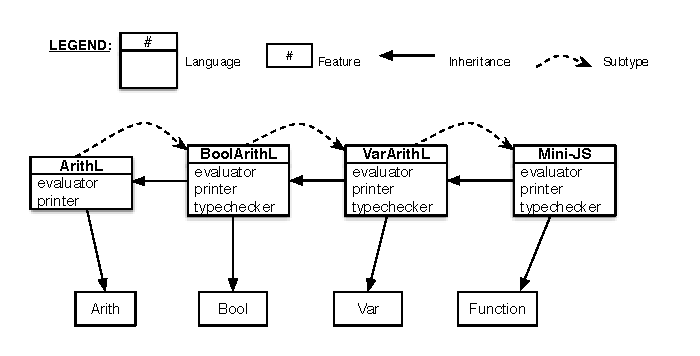
\includegraphics{dependency.eps}
%   \caption{Overview of the language components.}
%   \label{fig:dependency}
% \end{figure}

\subsection{Evaluation}
\label{sec:evaluate}

To evaluate \name's implementation of the case study,
\Cref{fig:sloc} compares the number of source lines of code
(SLOC, lines of code without counting empty lines and comments) for
\name's \emph{modular} implementation with the vanilla
\emph{non-modular} AST-based implementations in Haskell. The Haskell
implementations are just straightforward AST interpreters, which duplicate code across the multiple language
components.

Since \name is a new language, we
had to write various code that is provided in Haskell by the standard library,
so they are not counted for fairness of comparison. In the left part, for each
feature, we count the lines of the algebra interface (number beside the feature
name), and the algebras for the operations. In the right part, for each
language, we count the lines of ASTs, and those to combine previously
defined operations. For example, here is the code that is needed to make the
\lstinline{arith} language.
\lstinputlisting[linerange=537-544]{../../examples/case_study.sl}% APPLY:linerange=ARITH
We only need 8 lines in total: 2 lines for the AST, and 6 lines to combine the operations.

Therefore, the total SLOC of \name's implementation is the sum of all the
lines in the feature and language parts (237 SLOC of all features plus 94 SLOC
of ASTs and operations). Although \name is considerably more verbose than a
functional language like Haskell, \name's modular implementation for 12 languages and 30
operations in total reduces approximately 60\% in terms of SLOC. The reason is
that, the more frequently a feature is reused by other languages directly or
indirectly, the more reduction we see in the total SLOC. For example,
$\mathit{natF}$ is used across many languages. Even though \lstinline{simplenat}
itself \emph{alone} has more SLOC ($40 = 7+23+7+3$) than that of Haskell (which
has 33), we still get a huge gain when implementing other languages.

Finally, we acknowledge the limitation of our case study in that SLOC is just
one metric and we have not measured any other metrics. Nevertheless we believe
that the case study is already non-trivial in that we need to solve EP. Note
that Scala traits alone are not sufficient on their own to solve EP. While there
are solutions to EP in both Haskell and Scala, they
introduce significant complexity, as explained in \cref{sec:ob}.



\begin{figure}[t]
  \centering
  \begin{small}
  \begin{tabular}{|r|ccc||l|ccc|}
    \hline
     Feature & \textbf{eval} & \textbf{print} & \textbf{check} & Lang name & \name & \textbf{Haskell} & \textbf{\% Reduced}  \\
    \hline
    $\mathit{natF}$(7) & 23 & 7 & 39 & \lstinline$simplenat$ & 3 & 33 & 91\%  \\
    $\mathit{boolF}$(4) & 9 & 4 & 17 & \lstinline$simplebool$ & 3 & 16 & 81\% \\
    $\mathit{compF}$(4) & 12 & 4 & 20 & \lstinline$natbool$ & 5 & 74 & 93\% \\
    $\mathit{logicF}$(4) & 12 & 4 & 20 & \lstinline$varbool$ & 4 & 24 & 83\% \\
    $\mathit{varF}$(4) & 7 & 4 & 7 & \lstinline$varnat$ & 4 & 41 & 90\% \\
    $\mathit{funcF}$(3) & 10 & 3 & 9 & \lstinline$simplelogic$ & 4 & 28 & 86\% \\
     & & & & \lstinline$varlogic$ & 6 & 36 & 83\% \\
     & & & & \lstinline$arith$ & 8 & 94 & 91\% \\
     & & & & \lstinline$arithlogic$ & 8 & 114 & 93\% \\
     & & & & \lstinline$vararith$ & 8 & 107 & 93\% \\
     & & & & \lstinline$vararithlogic$ & 8 & 127 & 94\% \\
     & & & & \lstinline$mini-JS$ & 33 & 149 & 78\% \\
    \hline
    \bf{Total} & & & 237 & & 331 & 843 & 61\% \\
    \hline
  \end{tabular}
  \end{small}
  \caption{SLOC statistics: \name implementation vs vanilla AST implementation.}
  \label{fig:sloc}
\end{figure}




\begin{comment}
\subsection{Putting all together}

% With all the components ready, we can assemble them at will to cook a language
% with whatever features we want. For example, we hope by now the reader can share
% our feeling that this is indeed a simple and modular way to cook a language
% incrementally.

To demonstrate the usage of the final language \lstinline{MiniJS}, here is a function that
makes sure ``well-typed programs cannot go wrong'':
\lstinputlisting[linerange=-]{}% APPLY:linerange=SUPER_DEF
It type checks the program before passing it to the evaluator and pretty
printer.

% we first create a program that
% uses all the features the language supports now.
% \lstinputlisting[linerange=-]{}% APPLY:linerange=FINAL_TEST
% The concrete syntax of the program is shown in the comment above. We assume a
% pre-defined function environment (\lstinline{fenv}) containing the definition of
% the \lstinline{add1} function.

% Finally we apply it to the program we have just created:
% \lstinputlisting[linerange=735-736]{../../examples/case_study.sl}% APPLY:linerange=TEST_TEST
% Everything works as expected!
\end{comment}

\begin{comment}
\subsection{Parameterizing Expressions by the Evaluation Order}

We now turn to the second case study. In this case study, we embed a
higher-order domain-specific language inside \name. Our object language in this
case study is typed lambda calculus with conditional and constants. This time,
the embedding not only demonstrates the extensibility, as is shown in the first
case study, but also object types, expressed in the meta-language (\name) and
manifestly ensuring well-scoped and well-typed expressions in the object
language. What is more, the evaluator over the object expressions is type
preserving by construction. The embedding of typed languages is directly
inspired by Kiselyov's lecture notes~\cite{kiselyov2012typed} on the
"tagless-final" approach to embedding languages.

\paragraph{Well-typed object expressions} One important issue with such
embedding is how to deal with binders in the object language. In general there
are two options, one can either use deBrujin indices~\cite{}, or higher-order
abstract syntax (HOAS)~\cite{}. Each option has its cons and pros, but for this
particular case study, we find HOAS convenient. HOAS represents object language
abstractions as \name abstractions and object variables as \name variables. By
utilizing the infrastructure of the meta-language, we are free of issues such as
variable capture. Here is the interface of the object language.
\lstinputlisting[linerange=-]{}% APPLY:linerange=TYPED_LAMBDA
Embedded object expressions of type \lstinline{A} are represented as \name
values of the type \lstinline{Expr[A]}. The \lstinline{bot} constructor, which
represents non-terminating computation, is there for the purpose of illustrating
different evaluation strategies.

A careful reader may notice that the \lstinline{ExprAlg} interface has no
abstractions. This is intentional! Evaluators with different evaluation
strategies only differ in the interpretation for abstractions, as will be shown
later on. For this reason, \lstinline{lam} is moved to a separate interface of
its own.
\lstinputlisting[linerange=-]{}% APPLY:linerange=ABSTRACTION


\paragraph{Well-typed evaluator}
The benefit of typeful embedding shows up when defining the evaluator.
\lstinputlisting[linerange=-]{}% APPLY:linerange=TYPED_EVAL
Unlike the evaluator in the first case study, there is no need for a separate
\lstinline{Value} datatype for values, as they are directly modeled by \name
values. Note that the resulting evaluator is \emph{type preserving} by
construction.

\paragraph{Call-by-name, call-by-value}
Our evaluator defined in the first case study inherits the evaluation strategy
from the meta-language. We now show call-by-name and call-by-value evaluators.
The two evaluators are quite alike, sharing most of the code. As said before,
the only difference is the interpretation for \lstinline{lam}.
\lstinputlisting[linerange=-]{}% APPLY:linerange=CBN_CBV
The call-by-name \lstinline{lam}, when applied, will receive an unevaluated
argument expression, use it as it is. The call-by-value \lstinline{lam}, as in
the call-by-name evaluator, receives an unevaluated argument expression,
evaluates it before passing its result to the abstraction body \lstinline{f}.

Now to make an evaluator parameterized over the evaluation order, we just take a
trait \lstinline{o} with unknown implementation, compose it with other language
features.
\lstinputlisting[linerange=-]{}% APPLY:linerange=MAKE_EVAL
Here is the call-by-name evaluator at work:
\lstinputlisting[linerange=-]{}% APPLY:linerange=CBN_TEST
On the other hand, \lstinline{(evaluator evalBindCBV ex)()} would result in a
infinite loop. The complete code with several examples can be found in the
supplementary materials.

\jeremy{I am afraid we don't seem to have many advantages over OCaml's version,
  because we don't really have higher-kinded types, we cannot make a AST type
  for this example, though \lstinline{makeEvaluator} seems to be one advantage }

\end{comment}

%%% Local Variables:
%%% mode: latex
%%% TeX-master: "../paper"
%%% org-ref-default-bibliography: ../paper.bib
%%% End:


% \section{Desugaring}
\label{sec:desugar}

\name is built upon a thin-layer of sugar on top of
\bname~\cite{alpuimdisjoint}. \bname is a polymorphic language with subtyping,
and it was developed as an alternative to languages such as System $F_{<:}$ to
serve as a core language for OO languages. The choice of \bname is due to its
support for disjoint intersection types and disjoint polymorphism (used to model
subtyping and conflict detection), and the so-called merge construct (which is
used to model dynamic trait inheritance). The theoretical aspects of \bname
(including the formalization of the static and dynamic semantics, and the proofs
of type safety and coherence) were already studied in previous work. So they are
not a contribution of this paper and are not necessary to understand the
desugaring process.

The novelty in this section is to explain how to build a high-level OO
abstractions on top of the core constructs of \bname. In particular we focus on
how the trait system presented in this paper is built. The key idea behind trait
translation is inspired by the functional mixin semantics using open recursion,
which is proposed by~\citet{cook1989denotational} in an untyped setting.
However, our translation is done in the context of a statically-typed
programming language, which is exactly why conflicts can be \textit{statically}
detected in traits.

\subsection{A Brief Introduction to \bname}
The syntax of our core language \bname is shown in Figure~\ref{fig:synax-fi}.

\paragraph{Types}
Apart from normal type constructs, the main novelty are two constructs used to
support disjoint intersection types and disjoint polymorphism: intersection
types $[[A & B]]$ and disjoint (universal) quantification $[[ forall ( a ** A )
. B ]]$. \bname also includes singleton record types $[[{ l : A}]]$ and type
applications $[[ T [ B1 , .. , Bn ] ]]$.

\paragraph{Terms}
In correspondence with types, terms include merges $[[E1 ,, E2]]$, abstraction
of type variables over terms $[[blam ( a ** A ) . E]]$, applications of terms to
types $[[E A]]$, and singleton records $[[ { l = E } ]]$. Record operations are
projections $[[E.l]]$ and exclusions $[[E -- { l : A }]]$. We also have
recursive \lstinline{let} bindings.

\paragraph{Type and term declarations}

For the convenience of writing large programs, we also support type and term
declarations. A type declaration declares a type constructor's name $T$, its
type parameters and its definition $A$. A term declaration declares a function's
name $f$, its parameter signatures, its result type $B$, and its function body
$e$. Although previous work does not have declarations, we do not think adding
them will cause any problems to the meta-theory of \bname. A careful study of
these additions is of course a good avenue for future work.

\paragraph{Syntactic sugar} Multi-field record types are encoded as
intersections of singleton record types, and multi-field records as merges of
singleton records.

% \bruno{I think we can omit most of the primitive types and operations
%   from the formal syntax. You should present the syntactic sugar for
%   (multi-field) records and record types in the figure.}
% \bruno{Briefly explain the key novel contructs: merge, big lambda }
% \bruno{Explain that declarations/programs are new, but we don't think
%   this will cause any programs to the meta-theory.}

\begin{figure}[t]
\centering
\begin{small}
\begin{tabular}{lrcl}
  Types  & $[[A]], [[B]]$ & ::= & $[[top]] \mid [[Int]] \mid [[A -> B]] \mid [[A & B]] \mid  [[{ l : A }]] \mid [[a]] \mid [[forall ( a ** A ) . B]] \mid [[ T [ B1 , .. , Bn ] ]]$ \\
  Expressions & $[[E]]$ & ::= & $[[()]] \mid [[N]] \mid [[x]] \mid [[\ x . E]] \mid [[E1 E2]] \mid [[blam ( a ** A ) . E]] \mid [[E A]] \mid [[E1 ,, E2]] $ \\
         & & $\mid$ & $[[let x : A = E1 in E2]] \mid [[{ l = E }]] \mid [[E . l]] \mid [[E -- { l : A }]] $ \\
  Programs & $[[pgm]]$ & ::= & $[[decl1 .. decln E]]$ \\
  Declarations & $[[decl]]$ & ::= & $[[ def f ( x1 : A1 ) .. ( xn : An ) : B = E ]] \mid [[ type T [ a1 , .. , an ] = A ]]$ \\ \\
\end{tabular}
\begin{tabular}{llll}
  Record types & $[[ { l1 : A1 , ... , ln : An } ]] $ & := & $[[ { l1 : A1} & ... & { ln : An } ]]$ \\
  Records &  $[[ { l1 = E1 , ... , ln = En } ]] $ & := & $ [[ { l1 = E1 } ,, ... ,, { ln = En } ]]$
\end{tabular}
\end{small}
\caption{\bname syntax and syntactic abbreviations}
\label{fig:synax-fi}
\end{figure}

\subsection{Desugaring Traits}

\paragraph{Trait declarations}

The left part of Figure~\ref{fig:trans-trait} presents the translation of trait
declarations. Essentially traits are translated into term declarations, with
methods becoming record fields. The self-reference is adjusted to be the last
parameter of the declaration. For example
\lstinputlisting[linerange=13-13]{../examples/point.sl}% APPLY:linerange=DESUGAR1
becomes
\begin{lstlisting}
def point3D (x : Double) (y : Double) (self : Point3D) = point x y self ,, { z = self.x }
\end{lstlisting}
Now it is clear that \lstinline{self} is not a special keyword: it can have any
name.

% To account for the call-by-value semantics of the
% target language, the type of the self-reference $s$ has become a thunk
% \lstinline[mathescape=true]{T -> $A_0$}, and the occurrences of the
% self-reference \lstinline{s} in the trait body are replaced by \lstinline{s()}.


\paragraph{Instantiation of traits}

The right part of Figure~\ref{fig:trans-trait} shows the translation of trait
instantiation. Specifically, the self-reference gets passed to each trait $m_1$
to $m_n$, as each of them is an open term after translation. The results are
then merged to form a new term. \lstinline{new} instantiates a trait by
taking the \textit{lazy fixpoints} of the resulting term. For example,
\lstinline{new[Point3D] point3D(3,4)} is translated into \lstinline{let self : Point3D = point3D 3 4 self in self}.
% \name has a lazy (and possibly recursive) \lstinline{let} construct.


% Lazy fixpoints are implemented in \name using the built-in \lstinline{let}
% construct (possibly recursive), which employs call-by-name semantics. It is
% possible to choose call-by-value, then the type of the self-reference would
% become a thunk (e.g., \lstinline$T -> Point$) to prevent premature evaluation.


\paragraph{The type for traits}

\lstinline[mathescape=true]{Trait[$T_1, T_2$]} denotes the type of those traits
which provide an interface described by the type $T_2$ with dependency on $T_1$.
In fact, it is simply translated into $T_1 \rightarrow T_2$.

\begin{figure}[t]
  \centering
  \begin{tabular}{l|l}

\begin{lstlisting}[mathescape=true]
trait m ($x_1 : A_1$, ..., $x_n : A_n$)
  inherits $a_1$ & ... & $a_m$ { $s : A_0$ =>
  def $m_1$(..) = $e_1$
  ..
  def $m_s$(..) = $e_s$ }
\end{lstlisting} &

\begin{lstlisting}[mathescape=true]
new[A] $m_1$ & ... & $m_n$
\end{lstlisting}  \\

    $\rightsquigarrow$  & $\rightsquigarrow$ \\

\begin{lstlisting}[mathescape=true]
def m $(x_1 : A_1)$ ... $(x_n : A_n)$ $(s : A_0)$
  = $a_1$(s) ,, ... ,, $a_m$(s) ,,
{ $m_1$ = \(..) -> $e_1$
, ..
, $m_s$ = \(..) -> $e_s$ }
\end{lstlisting} &


\begin{lstlisting}[mathescape=true]
let self : A =
  $m_1$(self) ,, ... ,, $m_n$(self)
in self
\end{lstlisting}
  \end{tabular}
  \caption{Translations of trait declaration (left) and trait instantiation (right).}
\label{fig:trans-trait}

\end{figure}



\section{Implementation and Discussion}

\name implementation is done in Haskell, and is structured around a typed core language
(\bname with some extensions). The overall implementation is unremarkable, as it
closely follows the semantics presented by~\citet{alpuimdisjoint}. It consists
of 3 phases: 1) The desugaring phase (cf. Section~\ref{sec:desugar}) takes an
abstract syntax tree (AST) generated by the parser, and returns a \bname
expression. Trait-related constructs disappear after this phase; 2) the type
checking phase then takes a \bname expression from the previous phase, it infers
and checks its type, and in the meantime, produces an expression in the target
language; and 3) the target expression (call-by-name pure untyped lambda
calculus) then enters the final phase, and is executed by a simple interpreter.

% The main component of the implementation is an
% elaborating type-checker, which takes a \bname expression, checks it, and
% produces another expression in the target language. The final expression is then
% directly executed by an interpreter. We chose call-by-value untyped lambda
% calculus as the target language. Since we focus on the implementation, and types
% are irrelevant after type checking, the untyped lambda calculus is a suitable choice
% with minimal syntax.


The type checker is the most involved component in the pipeline. It contains a
(coercive) subtyping procedure and a disjointness checker, both of which are the
most critical parts in \name. In regard to the subtyping rules, in addition to what have
been presented~\citep{alpuimdisjoint}, we have an additional rule, which we
found helpful for enabling the composition of Object Algebras. For brevity, we
only show a simplified version below: \ottusedrule{\ottdruleSubXXR{}} By this
rule, one can derive for example,
$$
[[ { l : Int -> String} & { l : Bool -> Bool}]] <: [[ { l : Int & Bool -> String & Bool}]]
$$
We believe this rule would not endanger the type
system, as it is orthogonal to the other subtyping rules. Besides, our
preliminary meta-theory study shows that the new subtype system enjoys the same
properties as before.

% The prototype implementation is written in just 1400 lines of Haskell code.

% \begin{figure}[t]
%   \centering
%   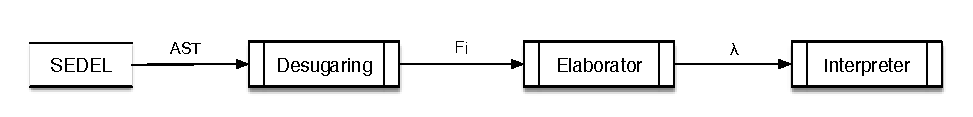
\includegraphics[scale=0.9]{pipeline.eps}
%   \caption{The pipeline of \name}
%   \label{fig:pipeline}
% \end{figure}

% 
\section{Discussion}
\label{sec:discuss}

Discuss the limitations/issues of \name. The differences from the original trait model.

\begin{itemize}
\item Override: Form a new trait by layering additional methods over an existing
  trait. This operation is an asymmetric sum.
\item Exclusion: forms a new trait by removing a method from an existing trait
\end{itemize}


\begin{itemize}
\item Traits have no proper notation of inheritance relationship (no super keyword)
\item Traits have no nice syntax of redefining
\item traits allow annotation of type, then term declarations don't need to
\end{itemize}

\section{Related Work}
\label{sec:related}

% \bruno{I think (part of) this text can be discussed in here instead:


There are multiple flavours of inheritance. To avoid confusion, since the same
terminology is often used in the literature to mean different things, we use the
following 3 terms when comparing related work with ours.

\begin{itemize}
\item{{\bf Static inheritance:}} Static inheritance refers to what the typical
  model of inheritance in class-based languages. The inheritance model is said
  to be static because when using class extension, the extended classes are
  statically known at compile-time.
\item{{\bf Mutable Inheritance:}} Prototype-based languages allow another model
  of inheritance, which we call \emph{mutable inheritance}. In this inheritance
  model, self-references are mutable and changeable at any point.
\item{{\bf Dynamic Inheritance:}} Dynamic inheritance is a less well-known model
  which stands in between static and mutable inheritance. Unlike the static
  inheritance model, with dynamic inheritance objects can inherit from other
  objects which are not statically known. However, unlike mutable inheritance,
  the self-reference is not mutable and cannot be arbitrarily changed at
  run-time.
\end{itemize}

Figure~\ref{fig:comparision} shows the comparison between \name and various
similar languages that follow \citeauthor{cook1989inheritance}'s ``Inheritance is not
Subtyping'' (i.e. the flexible model), as we will explain below.

\begin{figure}[t]
  \centering
  \begin{small}
  \begin{tabular}{|l||c|c|c|c|}
    \hline
    & \bf{Statically typed} & \bf{Polymorphism} & \bf{Meta-theory} & \bf{Inheritance}  \\
    \hline
    \name & \cmark & \cmark & \cmark & Dynamic \\
    \hline
    \textsc{Self} & \xmark & \xmark & \xmark & Mutable \\
    \hline
    Cecil & \cmark & \cmark & \xmark & Static \\
    \hline
    Cook's Modula-3 & \cmark & \xmark & \xmark & Static \\
    \hline
    IFJ & \cmark & \xmark & \cmark & Dynamic \\
    \hline
    \textsc{Darwin} & \cmark & \xmark & \xmark & Dynamic \\
    \hline
  \end{tabular}
  \end{small}
  \caption{Comparison between \name and various similar languages that
  adopt the \emph{flexible model}.}
  \label{fig:comparision}
\end{figure}



% \paragraph{Dynamically-typed Languages with Delegation Mechanism}

% \begin{itemize}
% \item Clojure Protocols
%   % http://www.ibm.com/developerworks/library/j-clojure-protocols/
% \item Ruby mixin
% \item JS mixin
% \end{itemize}

% They are all dynamically typed.


\paragraph{Delegation-based languages}

\citet{lieberman1986using} is the first to promote the use of prototypes and
delegation as the mechanism to code sharing between objects. Since then many
researchers have studied the mechanisms of
delegation~\cite{wegner1987dimensions,malenfant1995semantic,goldberg1989smalltalk}.
\textsc{Self}~\cite{ungar1988self} is a dynamically typed, prototype-based
language with a simple and uniform object model. \textsc{Self}'s inheritance
model is typical of what we call mutable inheritance, because an object's parent
slots may be assigned new values at run-time. Mutable inheritance is rather
unstructured, and oftentimes access to any clashing methods will generate a
``messageAmbiguous'' error at run-time. Although \name's dynamic inheritance is
not as powerful as mutable inheritance, its static type system can guarantee
that no such errors occur at run-time.

There is not much work on statically-typed, delegation-based languages.
\citet{kniesel1999type} provides a good overview of problems when combining
delegation with a static type discipline. Cecil~\cite{chambers1992object,
  chambers1993cecil} is a prototype-based language, where delegation is the
mechanism for method call and code reuse. Cecil supports a polymorphic static
type system, although no meta-theory of any kind is given. Its type system is
able to detect statically when a message might be ambiguously defined as a
result of multiple inheritance or multiple dispatching. However, one major
omission of Cecil, which is also one of the interesting features of \name, is
dynamic inheritance. There are other
works~\cite{fisher1995delegation,anderson2003can} on delegation in a
statically-typed setting, but none of them provide means (such as the merge
construct, disjointness constraints, etc.) that are needed for extensible
designs.

\citet{cook1989inheritance} were the first to propose a typed model of
inheritance where subtyping and inheritance are two separate concepts. In
particular, they introduce the notion of \textit{type inheritance} and show that
inherited objects have inherited types, not subtypes. An interesting aspect of
their calculus is the \textbf{with} construct, used to join two records. This is
somewhat similar to our merge construct. However two major differences are worth
pointing out: 1) the \textbf{with} construct operates only on records; and 2) it
is a biased operator, favoring values from its right argument. This biased
operator is good for modelling mixins, but not traits. The
\textbf{with} construct seems to be unable to merge two arbitrary (and possible
polymorphic) values, since this seems to require something like
\emph{row polymorphism}~\cite{wand1987complete,wand1989type}, which is not available in their language.
The \textit{onion} construct in the Big Bang
language~\cite{palmer2015building,menon2012big} has a similar bias problem -- it is a
left-associative operator which gives rightmost precedence to one
implementation when conflicts exist.

\paragraph{Mixin-based inheritance}

Mixins have become very popular in many OO languages
~\cite{flatt1998classes,bono1999core, ancona2003jam}. \citeauthor{bracha1990mixin}'s
seminal paper~\citep{bracha1990mixin} extends Modula-3 with mixins. Mixins are subclasses parameterized
over a superclass, and used to produce a variety of classes with the same
functionality and behaviour. Mixin-based inheritance requires that mixins be
composed linearly, and as such, conflicts are resolved implicitly (mixins
appearing later overwrite all the identically named features of earlier mixins).
In comparison, the trait model in \name requires conflicts be resolved
explicitly. We want to emphasize that this conflict detection is essential in
expressing composition operators for Object Algebras, without running
into ambiguities.


\paragraph{Trait-based inheritance}

The seminar paper by \citet{scharli2003traits} introduced the ideas behind
traits, where they also documented an implementation of the trait
mechanism in a dynamically typed version of Smalltalk. Since then many
formalizations of traits have been
proposed~\cite{scharli2003traitsformal,ducasse2006traits,bettini2010prototypical}.
For example \citet{fisher2004typed} presented a statically-typed calculus that
models traits. Conflict detection is the hallmark of trait-based
inheritance, compared with mixin-based inheritance. One important difference
with \name is that those systems support \textit{classes} in addition to traits,
and consider the interaction between them, whereas \name is 
delegation based and the mechanism for code reuse is purely traits
(i.e., there are no classes in \name). The
deviation from traditional class-based models is not only because of its
simplicity, but also because we need a very \textit{dynamic} form of
inheritance, as has been elaborated throughout the paper.

Compared to the traditional trait mode, traits in \name have the following
differences: 1) traditional traits cannot be instantiated but only composed with
a class, whereas traits in \name can be instantiated directly; 2) traditional
traits cannot take constructor parameters whereas ours can; 3) the trait system
in \name lacks a proper notation of inheritance relationship. For example in the
traditional trait model, if the same method (i.e., from the same trait) is
obtained more than once via different paths, there is no conflict. This is not
the case in \name; and 4) traits in \name support dynamic
inheritance. 
%In the
%traditional trait model, when it comes to inheritance, the traits being
%inherited must be statically known.




% \citet{flatt1998classes} proposed MIXEDJAVA, an extension to a subset of
% sequential Java called CLASSICJAVA with mixins. In their model, mixins
% completely subsume the role of classes (classes are mixins that do not inherit
% any services). One interesting aspect in their system is that two identically
% named methods are allowed to coexist, and are resolved at run-time with run-time
% context information provided by the current \textit{view} of an object. In
% comparison, conflicts in \name are detected statically, and resolved by the
% programmers. Like \name, their model also enforces the distinction between
% implementation inheritance and subtyping.

% \citet{bono1999core} develop an imperative class-based calculus that provides a
% formal model for both single and mixin inheritance. Objects are represented by
% records and produced by instantiating classes. In their calculus, the class
% construct is extensible but not subtypable, while objects are subtypable but not
% extensible. Like \name, their system has a clean separation between subtyping
% and inheritance. Also, their type system does not have polymorphism.

% \citet{ancona2003jam} extends the Java language to support mixins, called Jam.
% Since Jam is an upward-compatible extension of Java 1.0, it is inheritantly a
% covariant mode. Unlike MIXEDJAVA, mixins can be only instantiated on classes,
% and there is no notion of mixin composition.


\begin{comment}

\begin{itemize}


\item ``Object-Oriented Multi-Methods in Cecil''

\item ``Dimensions of Object-Based Language Design''

\item ``On the Semantic Diversity of Delegation-Based Programming Languages''

\item ``Self: The power of simplicity''

\item ``Type-safe delegation for run-time component adaptation''

\item ``A delegation-based object calculus with subtyping''

\item ``Can Addresses be Types? (a case study: objects with delegation)''

\item ``Inheritance is not subtyping''


Mixins

\item ``mixin-based inheritance''

\item ``Classes and mixins''

\item ``A core calculus of classes and mixins''

\item ``A core calculus of higher-order mixins and classes''

\item ``Jam—Designing a Java Extension with Mixins''



\end{itemize}

Do they have polymorphic type systems? Do they support mutable self reference?

\end{comment}


\paragraph{Class-based languages with more advanced forms of inheritance}

Incomplete Featherweight Java (IFJ), proposed by \citet{bettini2008type}, is a
conservative extension of Featherweight Java with incomplete objects. Besides
standard classes, programmers can also define incomplete classes, whose
instances are incomplete objects. Incomplete objects can be composed (by object
composition) with complete objects, yielding new complete objects at run-time,
while ensuring statically that the composition is type-safe. Incomplete objects
are quite flexible, and support dynamic inheritance. However, object composition
in IFJ is quite restrictive, compared to \name, in that it can only compose an
incomplete object with a complete object. In that regard, and also because IFJ's
type system is not polymorphic, IFJ is unable to encode composition operators of
Object Algebras. \citet{kniesel1999type} showed that type-safe integration of
delegation with subtyping into a class-based model is possible, resulting in the
\textsc{Darwin} model. In \textsc{Darwin}, the type of the parent object must be
a declared class and this limits the flexibility of dynamic composition.
\citeauthor{ostermann2002dynamically}'s delegation
layers~\citep{ostermann2002dynamically} use delegation for doing dynamic
composition in a system with virtual classes. This is in contrast with most
other approaches that use class-based composition, but closer to the dynamic
composition that we use in \name.

There are many other class-based OO languages that are equipped with more
advanced forms of
inheritance~\cite{meyer1987eiffel,buchi2000generic,ostermann2001object}. Most of
them are heavyweight and are specific to classes. \name is object-centered, more
lightweight, and is dedicated to express extensible designs in a simpler way.


% Eiffel~\cite{meyer1987eiffel} is a class-based language that is based on the
% identification of classes with types and of inheritance with subtyping. Eiffel
% supports multiple inheritance, with the restriction that name collisions are
% considered programming errors, and ambiguities must be resolved explicitly by
% the programmer (by means of renaming). In this regard, \name is quite like
% Eiffel. However, the type system in \name is more lenient in that two
% identically named methods with different signatures can coexist without any
% problems.

% \citet{kniesel1999type} is the first to show that type-safe integration of
% delegation with subtyping into a class-based model is possible, resulting in the
% DARWIN model. In the DARWIN model, the type of the parent object must be a
% declared class and this limits the flexibility of dynamic composition, whereas
% in \name, the merge operator can merge/compose any objects. Another difference
% with \name lies in the conflict resolution, where DARWIN relies on method
% overriding with the assumption that the author of the overriding method is aware
% of the effect.

% Generic wrappers~\cite{buchi2000generic} supports aggregating objects at
% run-time. In their model, once a ``wrappee'' is assigned to a ``wrapper'', the
% wrappee is fixed. GBETA~\cite{ernst2000gbeta} has some dynamic features that are
% related to delegation. Like Generic wrappers, parents in GBETA are fixed at
% run-time.

% \citet{ostermann2001object} proposed compound references (CR) as a abstraction
% for object references, which provides explicit linguistic support for combining
% different composition properties on-demand. The model is statically typed, and
% decouples subtype declaration from implementation reuse.


% \citet{ostermann2002dynamically} proposed delegation layers as an approach to
% decompose a collaboration into layers and compose these layers dynamically at
% run-time. This combines and generalizes delegation and virtual classes concepts.

% \citet{ostermann2008nominal} compared the nominal and structural subtyping
% mechanisms. They argue nominal subtyping gives more safety guarantee, whereas
% structural subtyping is more flexible from a component-based perspective. The
% type system of \name chooses structural subtyping.

\paragraph{Intersection types, polymorphism and the merge construct}

There is a large body of work on intersection types. Here we only talk about
work that have direct influences on ours. \citet{dunfield2014elaborating} shows
significant expressiveness of type systems with intersection types and a merge
construct. However his calculus lacks coherence. The limitation was addressed
by~\citet{oliveira2016disjoint}, where they introduced the notion of
disjointness to ensure coherence. The combination of intersection types, a merge
construct and parametric polymorphism, while achieving coherence was first
studied in the \bname calculus~\cite{alpuimdisjoint}, where they proposed the
notion of disjoint polymorphism. \bname serves as the theoretical foundation of
\name.


\begin{comment}

\begin{itemize}

\item Eiffel

\item ``Delegation by object composition'' (IFJ) and ``Type safe dynamic object
  delegation in class-based languages''

\item ``Dynamically composable collaborations with delegation layers''

\item ``Generic wrappers''

\item ``Object-Oriented Composition Untangled''

\item ``gbeta - a language with virtual attributes, Block Structure, and Propagating, Dynamic Inheritance''

\item ``Nominal and Structural Subtyping in Component-Based Programming''

\item ``Engineering a programming language: The type and class system of Sather ''

\item ``Big Bang Designing a Statically-Typed Scripting Language''

\item ``Building a Typed Scripting Language''



\end{itemize}

\end{comment}



\section{Conclusions and Future Work}
\label{sec:conclusion}

We have proposed \name, a type-safe and coherent calculus with disjoint
intersection types, and support for nested composition/subtyping. \name
improves upon earlier work with a more
flexible notion of disjoint intersection types, which leads to
a clean and elegant formulation of the type system. Due to the added
flexibility we have had to employ a more powerful proof method based on logical
relations to rigorously prove coherence.
We also show how \name supports essential features of family
polymorphism, such as nested composition. We believe \name provides insights into family polymorphism, and
has potential for practical applications for extensible software designs.

A natural direction for future work is to enrich \name with parametric
polymorphism. There is abundant literature on logical relations for parametric
polymorphism~\citep{reynolds1983types} and we foresee no fundamental
difficulties in extending our proof method.\footnote{
Our prototype
  implementation already supports polymorphism, but we
  are still in the process of extending our Coq development with polymorphism. } The resulting calculus will be
more expressive than \fname. An interesting application that we intend to investigate
is native support for \textit{object algebras}~\citep{oliveira2012extensibility}
(or the finally tagless approach~\citep{CARETTE_2009}). For example, we can
define the object algebra interfaces for the Expression Problem example in
\cref{sec:overview} as follows:
\lstinputlisting[linerange=75-76]{../../impl/examples/overview.sl}% APPLY:linerange=LANG_EXT_INTER
By instantiating \lstinline{E} with \lstinline{IPrint}, i.e.,
\lstinline{ExpAlg[IPrint]}, we get the interface of the \lstinline{Lang} family.
In that sense, object algebra interfaces can be viewed as family interfaces.
Moreover, combing algebras implementing \lstinline{ExpAlg[IPrint]} and
\lstinline{ExpAlg[IEval]} to form \lstinline{ExpAlg[IPrint & IEval]} is trivial
with nested composition. Polymorphism also improves code reuse across expressions in the
base and extended languages. For example, the following creates two expressions,
one in the base language, the other in the extended language:
\lstinputlisting[linerange=81-82]{../../impl/examples/overview.sl}% APPLY:linerange=LANG_EXT
Notice how we can  reuse \lstinline{e1} of the base language in the definition
of \lstinline{e2}.



% \jeremy{creating expressions using base and extended expressions, and show more reuse}

% \jeremy{future work} \jeremy{mention in passing this rule is unsound with
%   effects, see ``Intersection types and computational effects''}

% Local Variables:
% mode: latex
% TeX-master: "../paper"
% End:

%%
%% Bibliography
%%

%% Please use bibtex,

\bibliography{paper}


% \newpage
% \appendix
% \section{Full Specification of Core Language}

\subsection{Syntax}
\gram{\otte\ottinterrule
        \ottG\ottinterrule
        \ottv}
\\[2.0mm]
Syntactic Sugar\\
\resizebox{\columnwidth}{!}{$\ottcoresugar$} % defined in otthelper.mng.tex

\subsection{Operational Semantics}
\ottdefnstep{}
\ottusedrule{\ottdruleSXXMu{}}

\subsection{Typing}
\ottdefnctx{}\ottinterrule
\ottdefnexpr{}
\ottusedrule{\ottdruleTXXMu{}}

\section{Proofs about Core Language}
\subsection{Properties}
We follow the naming of lemmas and proofs of properties 
for Pure Type System from \cite{handbook}. Some lemmas have other well-known names, like
Lemma \ref{lem:appendix:thin} is often called \emph{Weakening} and 
Lemma \ref{lem:appendix:gen} is often called \emph{Inversion}.

\begin{comment}
\begin{lem}[Free Variable]\label{lem:appendix:free}
    If $[[G |- e:t]]$, then $\FV(e) \subseteq \dom([[G]])$ and $\FV([[t]])
\subseteq \dom([[G]])$.
\end{lem}

\begin{proof}
    By induction on the derivation of $[[G |- e:t]]$. We only treat cases
\ruleref{T\_Mu}, \ruleref{T\_CastUp} and \ruleref{T\_CastDown} (since proofs of
other cases are the same as \cc \cite{handbook}):
    \begin{description}
        \item[Case \ruleref{T\_Mu}:] From premises of $[[G |- (mu x:t.e1) :
t]]$, by the induction hypothesis, we have $\FV(e_1) \subseteq \dom([[G]]) \cup
\{[[x]]\}$ and $\FV(\tau) \subseteq \dom([[G]])$. Thus the result follows by
$\FV([[mu x:t.e1]])=\FV(e_1) \setminus \{[[x]]\} \subseteq \dom([[G]])$ and
$\FV(\tau) \subseteq \dom([[G]])$.
        \item[Case \ruleref{T\_CastUp}:] Since $\FV([[castup [t]
e1]])=\FV([[e1]])$, the result follows directly by the induction hypothesis.
        \item[Case \ruleref{T\_CastDown}:] Since $\FV([[castdown
e1]])=\FV([[e1]])$, the result follows directly by the induction hypothesis.
    \end{description}
\end{proof}
\end{comment}

\begin{lem}[Thinning]\label{lem:appendix:thin}
    Let $[[G]]$ and $[[G']]$ be legal contexts such that $[[G]] \subseteq
[[G']]$. If $[[G |- e : t]]$ then $[[G' |- e : t]]$.
\end{lem}

\begin{proof}
    By trivial induction on the derivation of $[[G |- e : t]]$.
\end{proof}

\begin{lem}[Substitution]\label{lem:appendix:subst}
	If $[[G1, x:T, G2 |- e1:t]]$ and $[[G1 |- e2:T]]$, then $[[G1, G2 [x |-> e2]
|- e1[x |-> e2]  : t[x |-> e2] ]]$.
\end{lem}

\begin{proof}
    By induction on the derivation of $[[G1, x:T, G2 |- e1:t]]$. We use the notation $[[e* == e
[x |-> e2] ]]$ to denote the substitution for short. Then the result can be written as \[ [[G1, G2* |- e1*  : t* ]]\]
We only treat cases \ruleref{T\_Mu}, \ruleref{T\_CastUp} and
\ruleref{T\_CastDown} since other cases can be easily followed by the proof for PTS in \cite{handbook}.
Consider the last step of derivation of the following
cases:
    \begin{description}
        \item[Case \ruleref{T\_Mu}:] $\inferrule{[[G1, x:T, G2, y:t |- e1:t]] \\
[[G1, x:T, G2 |- t:s]]}{[[G1, x:T, G2 |- (mu y:t.e1): t]]}$ 
        
        By the induction hypothesis, we have $[[G1, G2*, y:t* |- e1* : t*]]$ and $[[G1,
G2* |- t* : star]]$. Then by the derivation rule, $[[G1, G2* |- (mu
y:t*.e1*):t*]]$. Thus we can conclude $[[G1, G2* |- (mu y:t.e1)*:t*]]$.
        \item[Case \ruleref{T\_CastUp}:] $\inferrule{[[G1, x:T, G2 |- e1:t2]]
\\ [[G1, x:T, G2 |- t1:s]] \\ [[t1 --> t2]]}{[[G1, x:T, G2 |- (castup [t1]
e1):t1]]}$ 
        
        By the induction hypothesis, we have $[[G1, G2* |- e1*:t2*]]$, $[[G1, G2*
|- t1*:star]]$ and $[[t1 --> t2]]$. By the definition of substitution, we can
obtain $[[t1* --> t2*]]$ by $[[t1 --> t2]]$. Then by the derivation rule, $[[G1,
G2* |- (castup [t1*] e1*):t1*]]$. Thus we can conclude $[[G1, G2* |- (castup [t1]
e1)*:t1*]]$.
        \item[Case \ruleref{T\_CastDown}:] $\inferrule{[[G1, x:T, G2 |- e1:t1]]
\\ [[G1, x:T, G2 |- t2:s]] \\ [[t1 --> t2]]}{[[G1, x:T, G2 |- (castdown
e1):t2]]}$ 
        
        By the induction hypothesis, we have $[[G1, G2* |- e1*:t1*]]$, $[[G1, G2*
|- t2*:star]]$ and $[[t1 --> t2]]$ thus $[[t1* --> t2*]]$. Then by the
derivation rule, $[[G1, G2* |- (castdown e1*):t2*]]$. Thus we can conclude $[[G1, G2* |-
(castdown e1)*:t2*]]$.
    \end{description}
\end{proof}

\begin{lem}[Generation]\label{lem:appendix:gen}
If the alpha equivalence is witnessed by notation $[[=a]]$, we have the following results:
\begin{enumerate}[(1)]
	\item If $[[G |- x:T]]$, then there exist an expression $[[t]]$ such that $[[t
=a T]]$, $[[G |- t:s]]$ and $[[x:t elt G]]$.
	\item If $[[G |- e1 e2:T]]$, then there exist expressions $[[t1]]$ and
$[[t2]]$ such that $[[G |- e1 : (Pi x:t2.t1)]]$, $[[G |- e2:t2]]$ and $[[T =a
t1[x |-> e2] ]]$.
	\item If $[[G |- (\x:t1.e):T]]$, then there exist an expression $[[t2]]$ such
that $[[T =a Pi x:t1.t2]]$ where $[[G |- (Pi x:t1.t2):s]]$ and $[[G,x:t1 |-
e:t2]]$.
    \item If $[[G |- (Pi x:t1.t2):T]]$, then $[[T == s]]$, $[[G |- t1:s]]$ and
$[[G, x:t1 |- t2:s]]$.
	\item If $[[G |- (mu x:t.e):T]]$, then $[[G |- t:s]]$, $[[T =a t]]$ and $[[G,
x:t|-e:t]]$.
	\item If $[[G |- (castup [t1] e):T]]$, then there exist an expression $[[t2]]$
such that $[[G |- e:t2]]$, $[[G |- t1:s]]$, $[[t1 --> t2]]$ and $[[T =a t1]]$.
	\item If $[[G |- (castdown e):T]]$, then there exist expressions
$[[t1]],[[t2]]$ such that $[[G |- e:t1]]$, $[[G |- t2:s]]$, $[[t1 --> t2]]$ and
$[[T =a t2]]$.
\end{enumerate}
\end{lem}

\begin{proof}
    Consider a derivation of $[[G |- e:T]]$ for one of cases in the lemma. We
follow the process of derivation until expression $[[e]]$ is introduced the
first time. The last step of derivation can be done by
    \begin{itemize}
        \item rule \ruleref{T\_Var} for case 1;
        \item rule \ruleref{T\_App} for case 2;
        \item rule \ruleref{T\_Lam} for case 3;
        \item rule \ruleref{T\_Pi} for case 4;
        \item rule \ruleref{T\_Mu} for case 5;
        \item rule \ruleref{T\_CastUp} for case 6;
        \item rule \ruleref{T\_CastDown} for case 7.
    \end{itemize}
    In each case, assume the conclusion of the rule is $[[G' |- e : t']]$ where
$[[G']] \subseteq [[G]]$ and $[[t' =a T]]$. Then by inspection of used
derivation rules and Lemma \ref{lem:appendix:thin}, it can be shown that the
statement of the lemma holds and is the only possible case.
\end{proof}

\begin{lem}[Correctness of Types]\label{lem:appendix:corrtyp}
    If $[[G |- e:t]]$ then $[[t == s]]$ or $[[G |- t : s]]$.
\end{lem}

\begin{proof}
    Trivial induction on the derivation of $[[G |- e:t]]$ using Lemma
\ref{lem:appendix:gen}.
\end{proof}

\subsection{Decidability of Type Checking}
\begin{lem}[Decidability of One-step Reduction]\label{lem:appendix:unired}
	The one-step reduction $[[-->]]$ is called decidable if 
given $[[e]]$ there is a unique $[[e']]$ such that $[[e --> e']]$ or there is no such $[[e']]$.
\end{lem}

\begin{proof}
	By induction on the structure of $[[e]]$:
	\begin{description}
        \item[Case $[[e=x]]$:] $[[e]]$ is a variable which does not match any rules of $[[-->]]$. 
        Thus there is no $[[e]]'$ such that $[[e-->e']]$.
		\item[Case $[[e=v]]$:] $[[e]]$ is a value that has one of the following forms:
		\begin{inparaenum}[(1)]
		    \item $[[star]]$,
			\item $[[\x:t.e]]$,
			\item $[[Pi x:t1.t2]]$,
			\item $[[castup [t] e]]$.
		\end{inparaenum}
		Thus, it does not match any rules of $[[-->]]$. Then there is no $[[e]]'$ such that $[[e-->e']]$.
		\item[Case $[[e]]=[[(\x:t.e1) e2]]$:] Since the first term $[[\x:t.e1]]$ is a value, rule \ruleref{S\_App} does not apply to this case. Thus, only rule \ruleref{S\_Beta} can be applied and there is a unique $[[e']]=[[ e1[x|->e2] ]]$.
		\item[Case $[[e]]=[[castdown (castup [t] e1)]]$:] Since the inner term $[[castup [t] e1]]$ is a value, rule \ruleref{S\_CastDown} does not apply to this case. Thus, only rule \ruleref{S\_CastDownUp} can be applied and there is a unique $[[e']]=[[e1]]$.
		\item[Case $[[e]]=[[mu x:t.e1]]$:] Only rule \ruleref{S\_Mu} can be applied. Thus, there is a unique $[[e]]'=[[e1[x|->mu x:t.e1] ]]$.
		\item[Case $[[e]]=[[e1 e2]]$ and $[[e1]]$ is not a $\lambda$-term:] If
$[[e1]]=v$ and is not a $\lambda$-term, there is no rule to reduce $[[e]]$. 
Then there is no $[[e1']]$ such that $[[e1 --> e1']]$, which does not satisfy the premise of 
rule \ruleref{S\_App}. Thus, there is no $[[e]]'$ such that $[[e-->e']]$.

		Otherwise, if $[[e1]]$ is not a value, there exists some $[[e1']]$ such that $[[e1 --> e1']]$. By the
induction hypothesis, $[[e1']]$ is the unique reduction of $[[e1]]$. Thus, by rule
\ruleref{S\_App}, $[[e]]'=[[e1' e2]]$ is the unique reduction of $[[e]]$.
		\item[Case $[[e]]=[[castdown e1]]$ and $[[e1]]$ is not a $[[castup]]$-term:] If
$[[e1]]=v$ and is not a $[[castup]]$-term, there is no rule to reduce $[[e]]$. 
Then there is no $[[e1']]$ such that $[[e1 --> e1']]$, which does not satisfy the premise of 
rule \ruleref{S\_CastDown}. Thus, there is no $[[e]]'$ such that $[[e-->e']]$.

        Otherwise, if $[[e1]]$ is not a value, there exists some $[[e1']]$ such that $[[e1 --> e1']]$. By the
induction hypothesis, $[[e1']]$ is the unique reduction of $[[e1]]$. Thus, by rule
\ruleref{S\_CastDown}, $[[e]]'=[[castdown e1']]$ is the unique reduction of $[[e]]$.
	\end{description}
\end{proof}

\begin{thm}[Decidability of Type Checking]
	There is an algorithm which given $[[G]], [[e]]$ computes the unique
$[[t]]$ such that $[[G |- e:t]]$ or reports there is no such $[[t]]$.
\end{thm}

\begin{proof}
	By induction on the structure of $[[e]]$:
	\begin{description}
	    \item[Case $[[e=star]]$:] Trivial by applying \ruleref{T\_Ax} and $[[t ==
star]]$.
		\item[Case $[[e=x]]$:] Trivial by rule \ruleref{T\_Var}. If $[[x:t elt G]]$, then $[[t]]$ is the
unique type of $[[x]]$ such that $[[G |- x : t]]$. Otherwise, if $[[x]] \not \in \dom([[G]])$, there is no such $[[t]]$.
		\item[Case $[[e]]=[[e1 e2]]$:] By rule \ruleref{T\_App} and induction
hypothesis, there exist unique $[[t1]]$ and $[[t2]]$ such that $[[G
|- e1 : (Pi x:t1.t2)]]$, $[[G |- e2:t1]]$. Thus, $[[t2[x |-> e2] ]]$ is the unique type of $[[e]]$ such that $[[G |- e : t2[x |-> e2] ]]$.
		\item[Case $[[e=\x:t1.e1]]$:] By rule \ruleref{T\_Lam} and induction
hypothesis, there exist unique $[[t2]]$ such that $[[G |- (Pi
x:t1.t2):s]]$ and $[[G,x:t1 |- e:t2]]$. Thus, $[[Pi x:t1.t2 ]]$ is the unique type of $[[e]]$ such that $[[G |- e : Pi x:t1.t2  ]]$.
		\item[Case $[[e=Pi x:t1.t2]]$:] By rule \ruleref{T\_Pi} and induction
hypothesis, we have $[[G |- t1:s]]$ and $[[G, x:t1 |- t2:s]]$. Thus, $[[s]]$ is the unique type of $[[e]]$ such that $[[G |- e : s  ]]$.
		\item[Case $[[e=mu x:t.e1]]$:] By rule \ruleref{T\_Mu} and induction
hypothesis, we have $[[G |- t:s]]$ and $[[G, x:t|-e:t]]$. Thus, $[[t]]$ is the unique type of $[[e]]$ such that $[[G |- e : t]]$.
		\item[Case $[[e]]=[[castup [t1] e1]]$:] From the premises of rule
\ruleref{T\_CastUp}, by the induction hypothesis, we can derive the type of
$[[e1]]$ as $[[t2]]$ by $[[G |- e1:t2]]$, and check whether $[[t1]]$ is legal by $[[G |- t1:star]]$. 
For a legal $[[t1]]$, by Lemma \ref{lem:appendix:unired}, there is
a unique $[[t1']]$ such that $[[t1 --> t1']]$ or there is no such $[[t1']]$. 
If such $[[t1']]$ does not exist, then we report type checking fails. 

Otherwise, we examine if $[[t1']]$ is syntactically equal to $[[t2]]$, 
i.e., $[[t1' =a t2]]$. If the equality
holds, we conclude the unique type of $[[e]]$ is $[[t1]]$, i.e., $[[G |- e:t1]]$. Otherwise, we
report $[[e]]$ fails to type check.
		\item[Case $[[e]]=[[castdown e1]]$:] From the premises of rule
\ruleref{T\_CastDown}, by the induction hypothesis, we can derive the type of
$[[e1]]$ as $[[t1]]$ by $[[G |- e1:t1]]$. By Lemma \ref{lem:appendix:unired}, there is a unique
$[[t2]]$ such that $[[t1 --> t2]]$ or such $[[t2]]$ does not exist. 

If such $[[t2]]$ exists and its sorts is
$[[star]]$, we find the unique type of $[[e]]$ is $[[t2]]$ and can conclude $[[G |- e:t2]]$. Otherwise, we
report $[[e]]$ fails to type check.
	\end{description}
\end{proof}

\subsection{Type Safety}
\begin{dfn}[Multi-step reduction]
    The relation $[[->>]]$ is the transitive and reflexive closure of
$[[-->]]$.
\end{dfn}

\begin{dfn}[$n$-step reduction]
    The $n$-step reduction is denoted by $[[e0]] [[-->>]] [[en]]$, if
    there exists a sequence of one-step reductions $[[e0]] [[-->]]
    [[e1]] [[-->]] [[e2]] [[-->]] \dots [[-->]] [[en]]$, where $n$ is
    a positive integer and $[[ei]]\,(i=0,1,\dots,n)$ are valid
    expressions.
\end{dfn}

\begin{thm}[Subject Reduction]
If $[[G |- e:T]]$ and $[[e]] [[->>]] e'$ then $[[G |- e':T]]$.
\end{thm}

\begin{proof}
    We prove the case for one-step reduction, i.e., $[[e --> e']]$. The theorem
follows by induction on the number of one-step reductions of $[[e]] [[->>]]
[[e']]$.
    The proof is by induction with respect to the definition of one-step
reduction $[[-->]]$ as follows:
    \begin{description}
        \item[Case $\ottdruleSXXBeta{}$:] $\quad$ \\
        Suppose $[[G |- (\x:t1.e1)e2 :T]]$ and $[[G |- e1 [x |-> e2] :T']]$. By
Lemma \ref{lem:appendix:gen}(2), there exist expressions $[[t1']]$ and $[[t2]]$
such that 
        \begin{align}
            &[[G |- (\x:t1.e1):(Pi x:t1'.t2)]] \label{equ:lam} \\
            &[[G |- e2:t1']] \nonumber \\
            &[[T =a t2 [x |-> e2] ]] \nonumber
        \end{align}
        By Lemma \ref{lem:appendix:gen}(3), the judgement (\ref{equ:lam})
implies that there exists an expression $[[t2']]$ such that
        \begin{align}
            &[[Pi x:t1'.t2 =a Pi x:t1.t2']] \label{equ:lameq}\\
            &[[G, x:t1 |- e1:t2']] \nonumber
        \end{align}
        Hence, by (\ref{equ:lameq}) we have $[[t1 =a t1']]$ and $[[t2 =a
t2']]$. Then we can obtain $[[G, x:t1 |- e1:t2]]$ and $[[G |- e2:t1]]$. By
Lemma \ref{lem:appendix:subst}, we have $[[G |- e1[x |-> e2] : t2[x |-> e2]
]]$. Therefore, we conclude with $[[T' =a t2[x |-> e2] ]] [[=a]] [[T]]$.
        
        \item[Case $\ottdruleSXXApp{}$:] $\quad$ \\
        Suppose $[[G |- e1 e2 :T]]$ and $[[G |- e1' e2 :T']]$. By Lemma
\ref{lem:appendix:gen}(2), there exist expressions $[[t1]]$ and $[[t2]]$ such
that 
        \begin{align*}
            &[[G |- e1:(Pi x:t1.t2)]] \\
            &[[G |- e2:t1]]\\
            &[[T =a t2 [x |-> e2] ]]
        \end{align*}
        By the induction hypothesis, we have $[[G |- e1':(Pi x:t1.t2)]]$. By rule
\ruleref{T\_App}, we obtain $[[G |- e1' e2 : t2[x |-> e2] ]]$. Therefore, $[[T'
=a t2[x |-> e2] ]] [[=a]] [[T]]$.
        
        \item[Case $\ottdruleSXXCastDown{}$:] $\quad$ \\
        Suppose $[[G |- castdown e :T]]$ and $[[G |- castdown e' :T']]$. By
Lemma \ref{lem:appendix:gen}(7), there exist expressions $[[t1]], [[t2]]$ such
that 
        \begin{align*}
            &[[G |- e:t1]] \qquad [[G |- t2:s]] \\
            &[[t1 --> t2]] \qquad [[T =a t2 ]]
        \end{align*}
        By the induction hypothesis, we have $[[G |- e':t1]]$. By rule
\ruleref{T\_CastDown}, we obtain $[[G |- castdown e' : t2 ]]$. Therefore, $[[T'
=a t2]] [[=a]] [[T]]$.
        
        \item[Case $\ottdruleSXXCastDownUp{}$:] $\quad$ \\
        Suppose $[[G |- castdown (castup [t1] e) :T]]$ and $[[G |- e :T']]$. By
Lemma \ref{lem:appendix:gen}(7), there exist expressions $[[t1']], [[t2]]$ such
that 
        \begin{align}
            &[[G |- (castup [t1] e):t1']] \label{equ:fold} \\
            &[[t1' --> t2]] \label{equ:foldeq1} \\
            &[[T =a t2 ]] \label{equ:foldeq4}
        \end{align}
        By Lemma \ref{lem:appendix:gen}(6), the judgement (\ref{equ:fold})
implies that there exists an expression $[[t2']]$ such that
        \begin{align}
            &[[G |- e:t2']] \label{equ:foldr} \\
            &[[t1 --> t2']] \label{equ:foldeq2} \\
            &[[t1' =a t1]] \label{equ:foldeq3}
        \end{align}
        By (\ref{equ:foldeq1}, \ref{equ:foldeq2}, \ref{equ:foldeq3}) and Lemma
\ref{lem:appendix:unired} we obtain $[[t2 =a t2']]$. From (\ref{equ:foldr}) we
have $[[T' =a t2' ]]$. Therefore, by (\ref{equ:foldeq4}), $[[T' =a t2' ]]
[[=a]] [[t2 =a T]]$.
        
        \item[Case $\ottdruleSXXMu{}$:] $\quad$ \\
        Suppose $[[G |- (mu x:t.e) :T]]$ and $[[G |- e[x |-> mu x:t.e] :T']]$.
By Lemma \ref{lem:appendix:gen}(5), we have $[[T =a t]]$ and $[[G, x:t |-
e:t]]$. Then we obtain $[[G |- (mu x:t.e) : t]]$. Thus by Lemma
\ref{lem:appendix:subst}, we have $[[G |- e[x |-> mu x:t.e] : t[x |-> mu x:t.e]
]]$.
        
        Note that $[[x]]:[[t]]$, i.e., the type of $[[x]]$ is $[[t]]$, then
$[[x]] \notin \FV([[t]])$ holds implicitly. Hence, by the definition of
substitution, we obtain $[[t[x |-> mu x:t.e] == t]]$. Therefore, $[[T' =a t[x
|-> mu x:t.e] ]] [[==]] [[t =a T]]$.
    \end{description}
\end{proof}

\begin{thm}[Progress]
If $[[empty |- e:T]]$ then either $[[e]]$ is a value $v$ or there exists $[[e]]'$
such that $[[e --> e']]$.
\end{thm}

\begin{proof}
    By induction on the derivation of $[[empty |- e:T]]$ as follows:
    \begin{description}
        \item[Case $[[e=x]]$:] Impossible, because the context is empty.
        \item[Case $[[e=v]]$:] Trivial, since $[[e]]$ is already a value that
has one of the following forms:
		\begin{inparaenum}[(1)]
		    \item $[[star]]$,
			\item $[[\x:t.e]]$,
			\item $[[Pi x:t1.t2]]$,
			\item $[[castup [t] e]]$.
		\end{inparaenum}
		\item[Case $[[e]]=[[e1 e2]]$:] By Lemma \ref{lem:appendix:gen}(2), there
exist expressions $[[t1]]$ and $[[t2]]$ such that $[[empty |- e1:(Pi x:t1.t2)]]$ and
$[[empty |-e2:t1]]$. Consider whether $[[e1]]$ is a value:
    		\begin{itemize}
    		    \item If $[[e1]]=v$, by Lemma \ref{lem:appendix:gen}(3), it must be a
$\lambda$-term such that $[[e1 == \x:t1.e1']]$ for some $[[e1']]$ satisfying
$[[empty |- e1':t2]]$. Then by rule \ruleref{S\_Beta}, we have $[[(\x:t1.e1') e2 -->
e1' [x |-> e2] ]]$. Thus, there exists $[[e' == e1' [x |-> e2] ]]$ such that
$[[e --> e']]$.
    		    \item Otherwise, by the induction hypothesis, there exists $[[e1']]$ such
that $[[e1 --> e1']]$. Then by rule \ruleref{S\_App}, we have $[[e1 e2 --> e1'
e2]]$. Thus, there exists $[[e' == e1' e2]]$ such that $[[e --> e']]$.
    		\end{itemize}
		\item[Case $[[e]]=[[castdown e1]]$:] By Lemma \ref{lem:appendix:gen}(7),
there exist expressions $[[t1]]$ and $[[t2]]$ such that $[[empty |- e1:t1]]$ and
$[[t1 --> t2]]$. Consider whether $[[e1]]$ is a value:
		     \begin{itemize}
    		    \item If $[[e1]]=v$, by Lemma \ref{lem:appendix:gen}(6), it must be a
$[[castup]]$-term such that $[[e1 == castup [t1] e1']]$ for some $[[e1']]$
satisfying $[[empty |- e1':t2]]$. Then by rule \ruleref{S\_CastDownUp}, we can obtain
$[[castdown (castup [t1] e1') --> e1']]$. Thus, there exists $[[e' == e1']]$
such that $[[e --> e']]$.
    		    \item Otherwise, by the induction hypothesis, there exists $[[e1']]$ such
that $[[e1 --> e1']]$. Then by rule \ruleref{S\_CastDown}, we have $[[castdown
e1 --> castdown e1']]$. Thus, there exists $[[e' == castdown e1']]$ such that
$[[e --> e']]$.
    		\end{itemize}
		\item[Case $[[e]]=[[mu x:t.e1]]$:] By rule \ruleref{S\_Mu}, there always
exists $[[e' == e1[x |-> mu x:t.e1] ]]$.
    \end{description}
\end{proof}

\section{Full Specification of Surface Language}
\subsection{Syntax}
See Figure \ref{fig:appendix:syntax}.
\begin{figure*}
\centering
\gram{\ottpgm\ottinterrule
\ottdecl\ottinterrule
\ottu\ottinterrule
\ottp\ottinterrule
\ottE\ottinterrule
\ottGs}
\begin{align*}
&\text{Syntactic Sugar} \\
&\ottsurfsugar % defined in otthelper.mng.tex
\end{align*}
\caption{Syntax of the surface language}
\label{fig:appendix:syntax}
\end{figure*}

\subsection{Expression Typing}
See Figure \ref{fig:appendix:typing}.

\subsection{Translation to the Core}
See Figure \ref{fig:appendix:translate}.

\section{Proofs about Surface Language}
\subsection{Type Safety of the Translation}

\begin{thm}[Type Safety of Expression Translation]
Given a surface language expression $[[E]]$ and context $[[Gs]]$, 
if $[[Gs |- E:A ~> e]]$, $[[Gs |- A:star ~> t]]$ and $[[|- Gs ~> G]]$, then
$[[G |- e:t]]$.
\end{thm}

\begin{proof}
    By induction on the derivation of $[[Gs |- E : A ~> e]]$. Suppose there is
a core language context $[[G]]$ such that $[[|- Gs ~> G]]$.
    \begin{description}
        \renewcommand{\hlmath}[1]{#1}
        \item[Case $\ottdruleTRXXAx{}$:] $\quad$ \\ Trivial. $[[e]] = [[t]] = [[star]]$ and
$[[G |- star:star]]$ holds by rule \ruleref{T\_Ax}.
        \item[Case $\ottdruleTRXXVar{}$:] $\quad$ \\ Trivial. By rule \ruleref{T\_Var}, we
have $[[|- Gs ~> G]]$, then $[[x]]:[[t]] [[elt]] [[G]]$ where $[[Gs |-
A:star~>t]]$.
        \item[Case \resizebox{.9\columnwidth}{!}{$\ottdruleTRXXApp{}$}:] $\quad$ \\ Suppose
            \[\begin{array}{l}
            [[Gs |- E1 E2 : A1[x |-> E2] ~> e1 e2]] \\
            [[Gs |- A1[x |-> E2] : star ~> t1 [x |-> e2] ]].
            \end{array} \]
            By induction
            hypothesis, we have 
            $
            [[G |- e1 : (Pi x:t2.t1)]],
            [[G |- e2:t2]],
            $
            where
            \[\begin{array}{l}
             [[Gs |- E1 : (Pi x:A2.A1) ~> e1]] \\
              [[Gs |- (Pi x:A2.A1) : star ~> (Pi x:t2.t1)]] \\
              [[Gs |- E2 : A2 ~> e2]] \\
              [[Gs |- A2 : star ~> t2]].
            \end{array}\] Thus by rule \ruleref{T\_App}, we can conclude $[[G |- e1 e2 : t1 [x |-> e2] ]]$.
        \item[Case $\ottdruleTRXXLam{}$:] $\quad$ \\ Suppose
            \[\begin{array}{l}
            [[Gs |- (\x:A1.E):(Pi x:A1.A2) ~> \x:t1.e]] \\ 
            [[Gs |- Pi x:A1.A2 : star ~> Pi x:t1.t2]].
            \end{array} \]
            By the induction hypothesis, we have 
            $
            [[G, x : t1 |- e:t2]],
            [[G |- Pi x:t1.t2 : star]]
            $
            where 
            \[
            \begin{array}{ll}
            [[Gs, x : A1 |- E : A2 ~> e]] & \\
            [[Gs |- A1 : star ~> t1]] & [[Gs |- A2 : star ~> t2]] \\
            [[Gs |- (Pi x:A1.A2) : s ~> Pi x:t1.t2]] &
            \end{array}
            \]
            Thus by rule \ruleref{T\_Lam}, we can conclude $[[G |- (\x:t1.e):(Pi x:t1.t2)]]$.
        \item[Case $\ottdruleTRXXPi{}$:] $\quad$ \\ Suppose 
                \[ [[Gs |- (Pi x:A1.A2):r ~> Pi x:t1.t2]]. \] 
            By the induction hypothesis, we have 
            $
                [[G |- t1 : star]], [[G, x : t1 |- t2 : star]]
            $
            where
            $
                [[Gs |- A1 : s ~> t1]], [[Gs, x: A1 |- A2 : r ~> t2]]
            $
            Thus by rule \ruleref{T\_Pi} we can conclude $[[G |- (Pi x:t1.t2) : star]]$.
        \item[Case $\ottdruleTRXXMu{}$:] $\quad$ \\ Suppose 
                \[\begin{array}{l}
                    [[Gs |- (mu x:A . E):A ~> mu x:t.e]] \\
                    [[Gs |- A : star ~> t]]. 
                \end{array}\]
            By the induction hypothesis, we have 
                \[ [[G, x : t |- e : t]],\text{ where }[[Gs, x:A |- E:A ~> e]]. \] 
            Thus by rule \ruleref{T\_Mu}, we can conclude $[[G |- (mu x:t.e) : t]]$.
        \item[Case \resizebox{.9\columnwidth}{!}{$\ottdruleTRXXCase{}$}:] $\quad$ \\ Suppose 
            \[\begin{array}{l}
                [[Gs |- case E1 of << p => E2>> : B ~> (unfoldnp e1) T <<e2>>]] \\
                [[Gs |- B : star ~> T]].
            \end{array}\]
            By the induction hypothesis, we have 
            \[\begin{array}{ll}
                [[Gs |- E1 : D@<<U>>n ~> e1]] &
                [[Gs |- D@<<U>>n : star ~> t1]] \\
                [[G |- e1 : t1]] &
                [[<< Gs |- p => E2 : D@<<U>>n -> B ~> e2 >>]]            
            \end{array}\]
            By rule \ruleref{TRpat\_Alt}, we have
            \begin{align*}
                [[p]] &[[==]] [[K <<x:A[<< u |-> U >>]>>]] \\
                [[<<e2>>]] &[[==]] [[<<\ <<x:t'>> .e>>]]
            \end{align*}
            where
            \[\begin{array}{ll}
                [[<<Gs |- E2 : B ~> e>>]] &
                [[<<G |- e : T>>]] \\
                [[<<Gs |- U : star ~> uu'>>]] &
                [[<<Gs |- A[<< u |-> U >>]:star ~> t[<<uu |-> uu'>>]>>]] \\
                [[t']] [[==]] [[ t[<<uu |-> uu'>>] ]]
            \end{array}\]
            By rule \ruleref{TRdecl\_Data}, we have $[[D]]  [[ == ]] \ottdeclD$. Thus,
            \[ [[t1]] [[==]] [[D]] [[<<uu'>>]]^n,\text{ where }[[<<G |- uu' : ro>>]].\] 
            Note that by operational semantics of \name, the following reduction sequence follows for $[[t1]]$:
            \begin{align*}
                [[D]] [[<<uu'>>]]^n~
                &[[-->]]~ \mathscale[0.7]{[[(\ <<u:ro>>n . (bb:star) -> << ((<<x : t[D |-> X][X |-> D]>>) -> bb) >> -> bb) ]][[<<uu'>>]]^n}\\
                &[[-->>]]~ [[(bb:star) -> << (<<x:t'>>) -> bb >> -> bb]]
            \end{align*}
            Then by
            rule \ruleref{T\_CastDown} and the definition of $n$-step cast operator, the
            type of $[[unfoldnp e1]]$ is \[ [[(bb:star) -> << (<<x:t'>>) -> bb >> -> bb]].\] Note
            that by rule \ruleref{T\_Lam}, $[[G |- e2 : (<<x:t'>>) -> T]]$. Therefore, by rule
            \ruleref{T\_App}, we can conclude $[[G |- (unfoldnp e1) T <<e2>> : T]]$.
    \end{description}
\end{proof}

\begin{figure*}
\renewcommand{\hlmath}[1]{}
\renewcommand{\ottdrulename}[1]{\textsc{\replace{#1}{TR}{TS}}}
\renewcommand{\ottcom}[1]{\text{\replace{#1}{translation}{typing}}}
\ottdefnctxtrans{}\ottinterrule
\ottdefnpgmtrans{}\ottinterrule
\ottdefndecltrans{}\ottinterrule % defined in otthelper.mng.tex
\ottdefnpattrans{}\ottinterrule
\ottdefnexprtrans{}
\caption{Typing rules of the surface language}
\label{fig:appendix:typing}
\end{figure*}

\begin{figure*}
\ottdefnctxtrans{}\ottinterrule
\ottdefnpgmtrans{}\ottinterrule
\ottdefndecltrans{}
\[\hlmath{\ottdecltrans}\]\ottinterrule % defined in otthelper.mng.tex
\ottdefnpattrans{}\ottinterrule
\ottdefnexprtrans{}
\caption{Translation rules of the surface language}
\label{fig:appendix:translate}
\end{figure*}







\end{document}
